\section{Exigences fonctionnelles des protections}
Cette section a pour but de détailler les différentes exigences que les deux protections vont devoir remplir.

Les protections :
\begin{enumerate}
    \item Assureront une protection complète contre les réflexions du laser, afin de garantir la sécurité des utilisateurs du kit.
    \item Ne devront pas restreindre l'accessibilité des autres composants, tels que les lentilles réglables ainsi que le laser, afin de pouvoir régler ceux-ci facilement si nécessaire.
    \item Seront des assemblages mécaniques simples à monter et à démonter.
    \item Auront une conception simple, afin que leur fabrication soit la plus aisée possible.
    \item Comprendront le moins de pièces et de visseries possible.
\end{enumerate}


\begin{minipage}{\textwidth}
    \section{Protection à l'entrée du laser}
    Dans cette partie, les différentes étapes seront expliquées; la conception de la protection à l'entrée du laser, la modélisation de celle-ci, les prototypes qui ont été réalisés, la fabrication final ainsi que le montage.

    \subsection{Prototype initial en carton}
    Lorsqu'il est possible de faire un prototype en carton, je le fais afin d'avoir une première idée concrète du projet à réaliser. Ses avantages résident dans le fait que c'est rapide à créer et simple. La première idée a directement été une boîte qui entoure la cage de lentille avec un système de capot qui peut se soulever. Ci-dessous, deux photos du prototype en carton, avec une photo où le capot est fermée, voir Figure \ref{carton_protection_fermee}, et également une photo quand la protection est ouverte, voir Figure \ref{carton_protection_ouverte}.

    \vspace{2em}
    \begin{minipage}[c]{0.48\textwidth}
        \begin{center}
            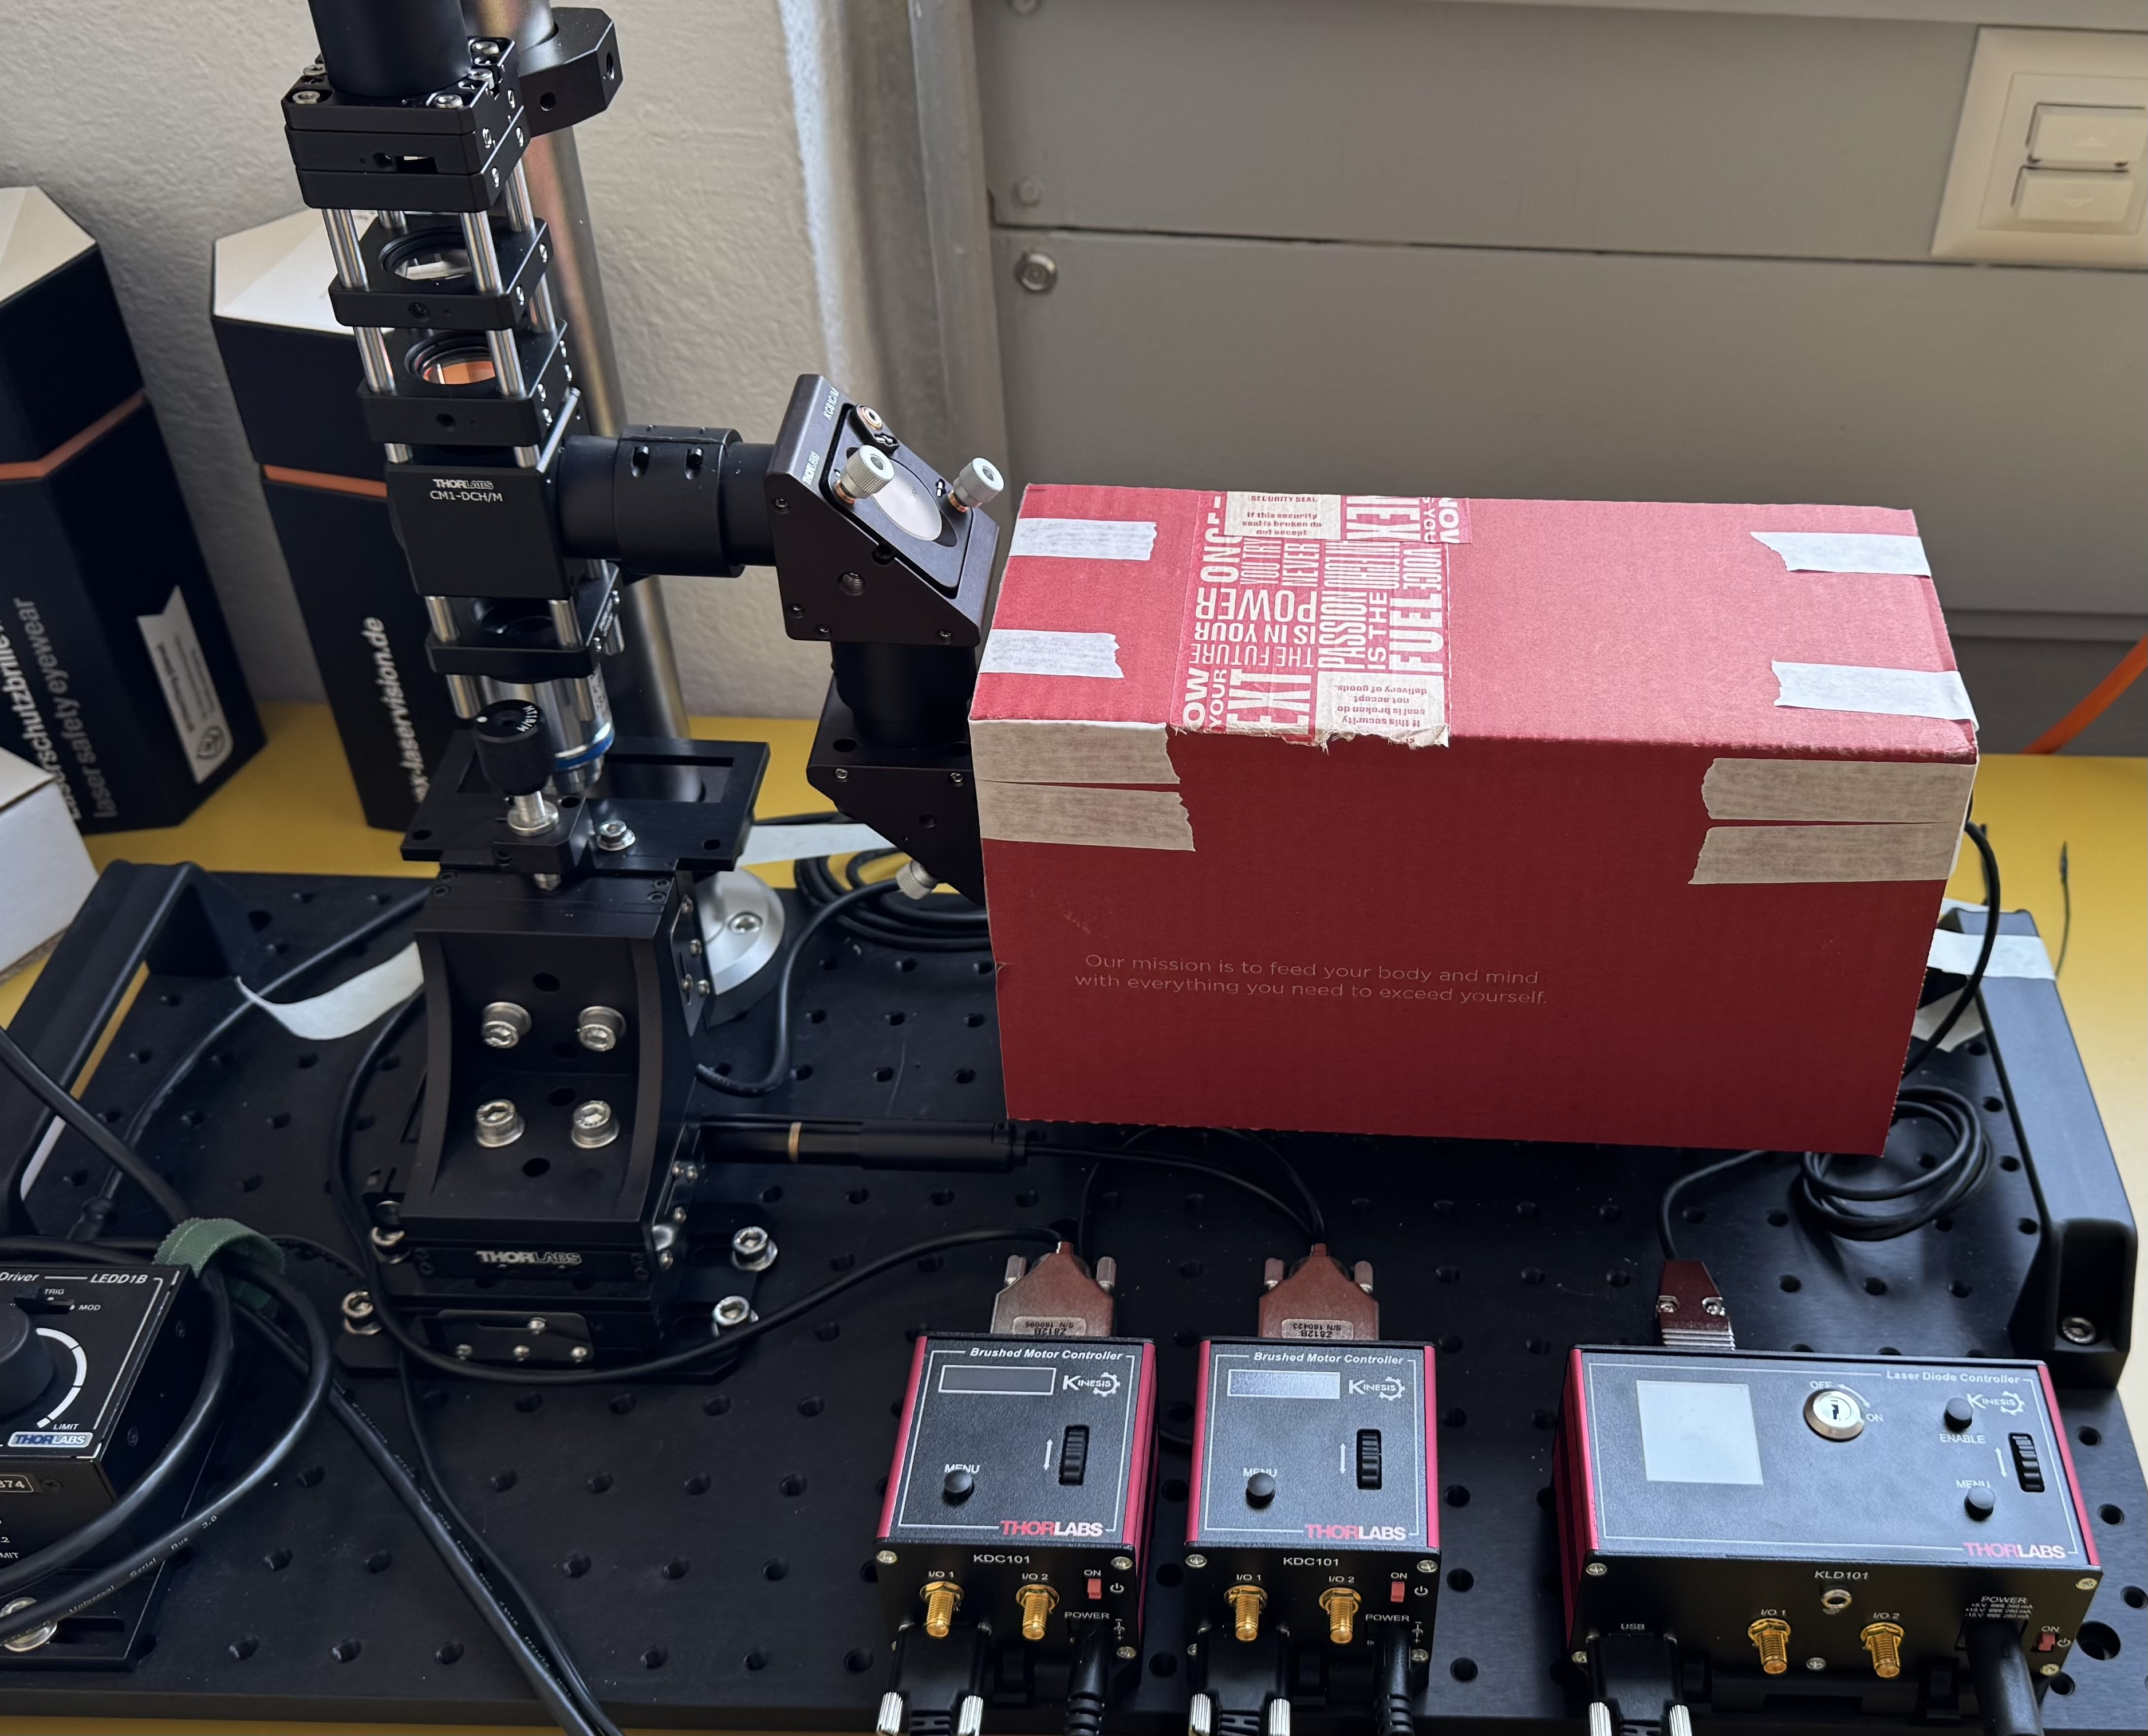
\includegraphics[width=\textwidth]{assets/figures/Protections_laser/Securite_mecanique/Protection_entree_laser/carton_protection_ferme.jpeg}
        \end{center}
        \captionof{figure}{Prototype en carton, protection fermée}
        \label{carton_protection_fermee}
    \end{minipage}\hfill
    \begin{minipage}[c]{0.48\textwidth}
        \begin{center}
            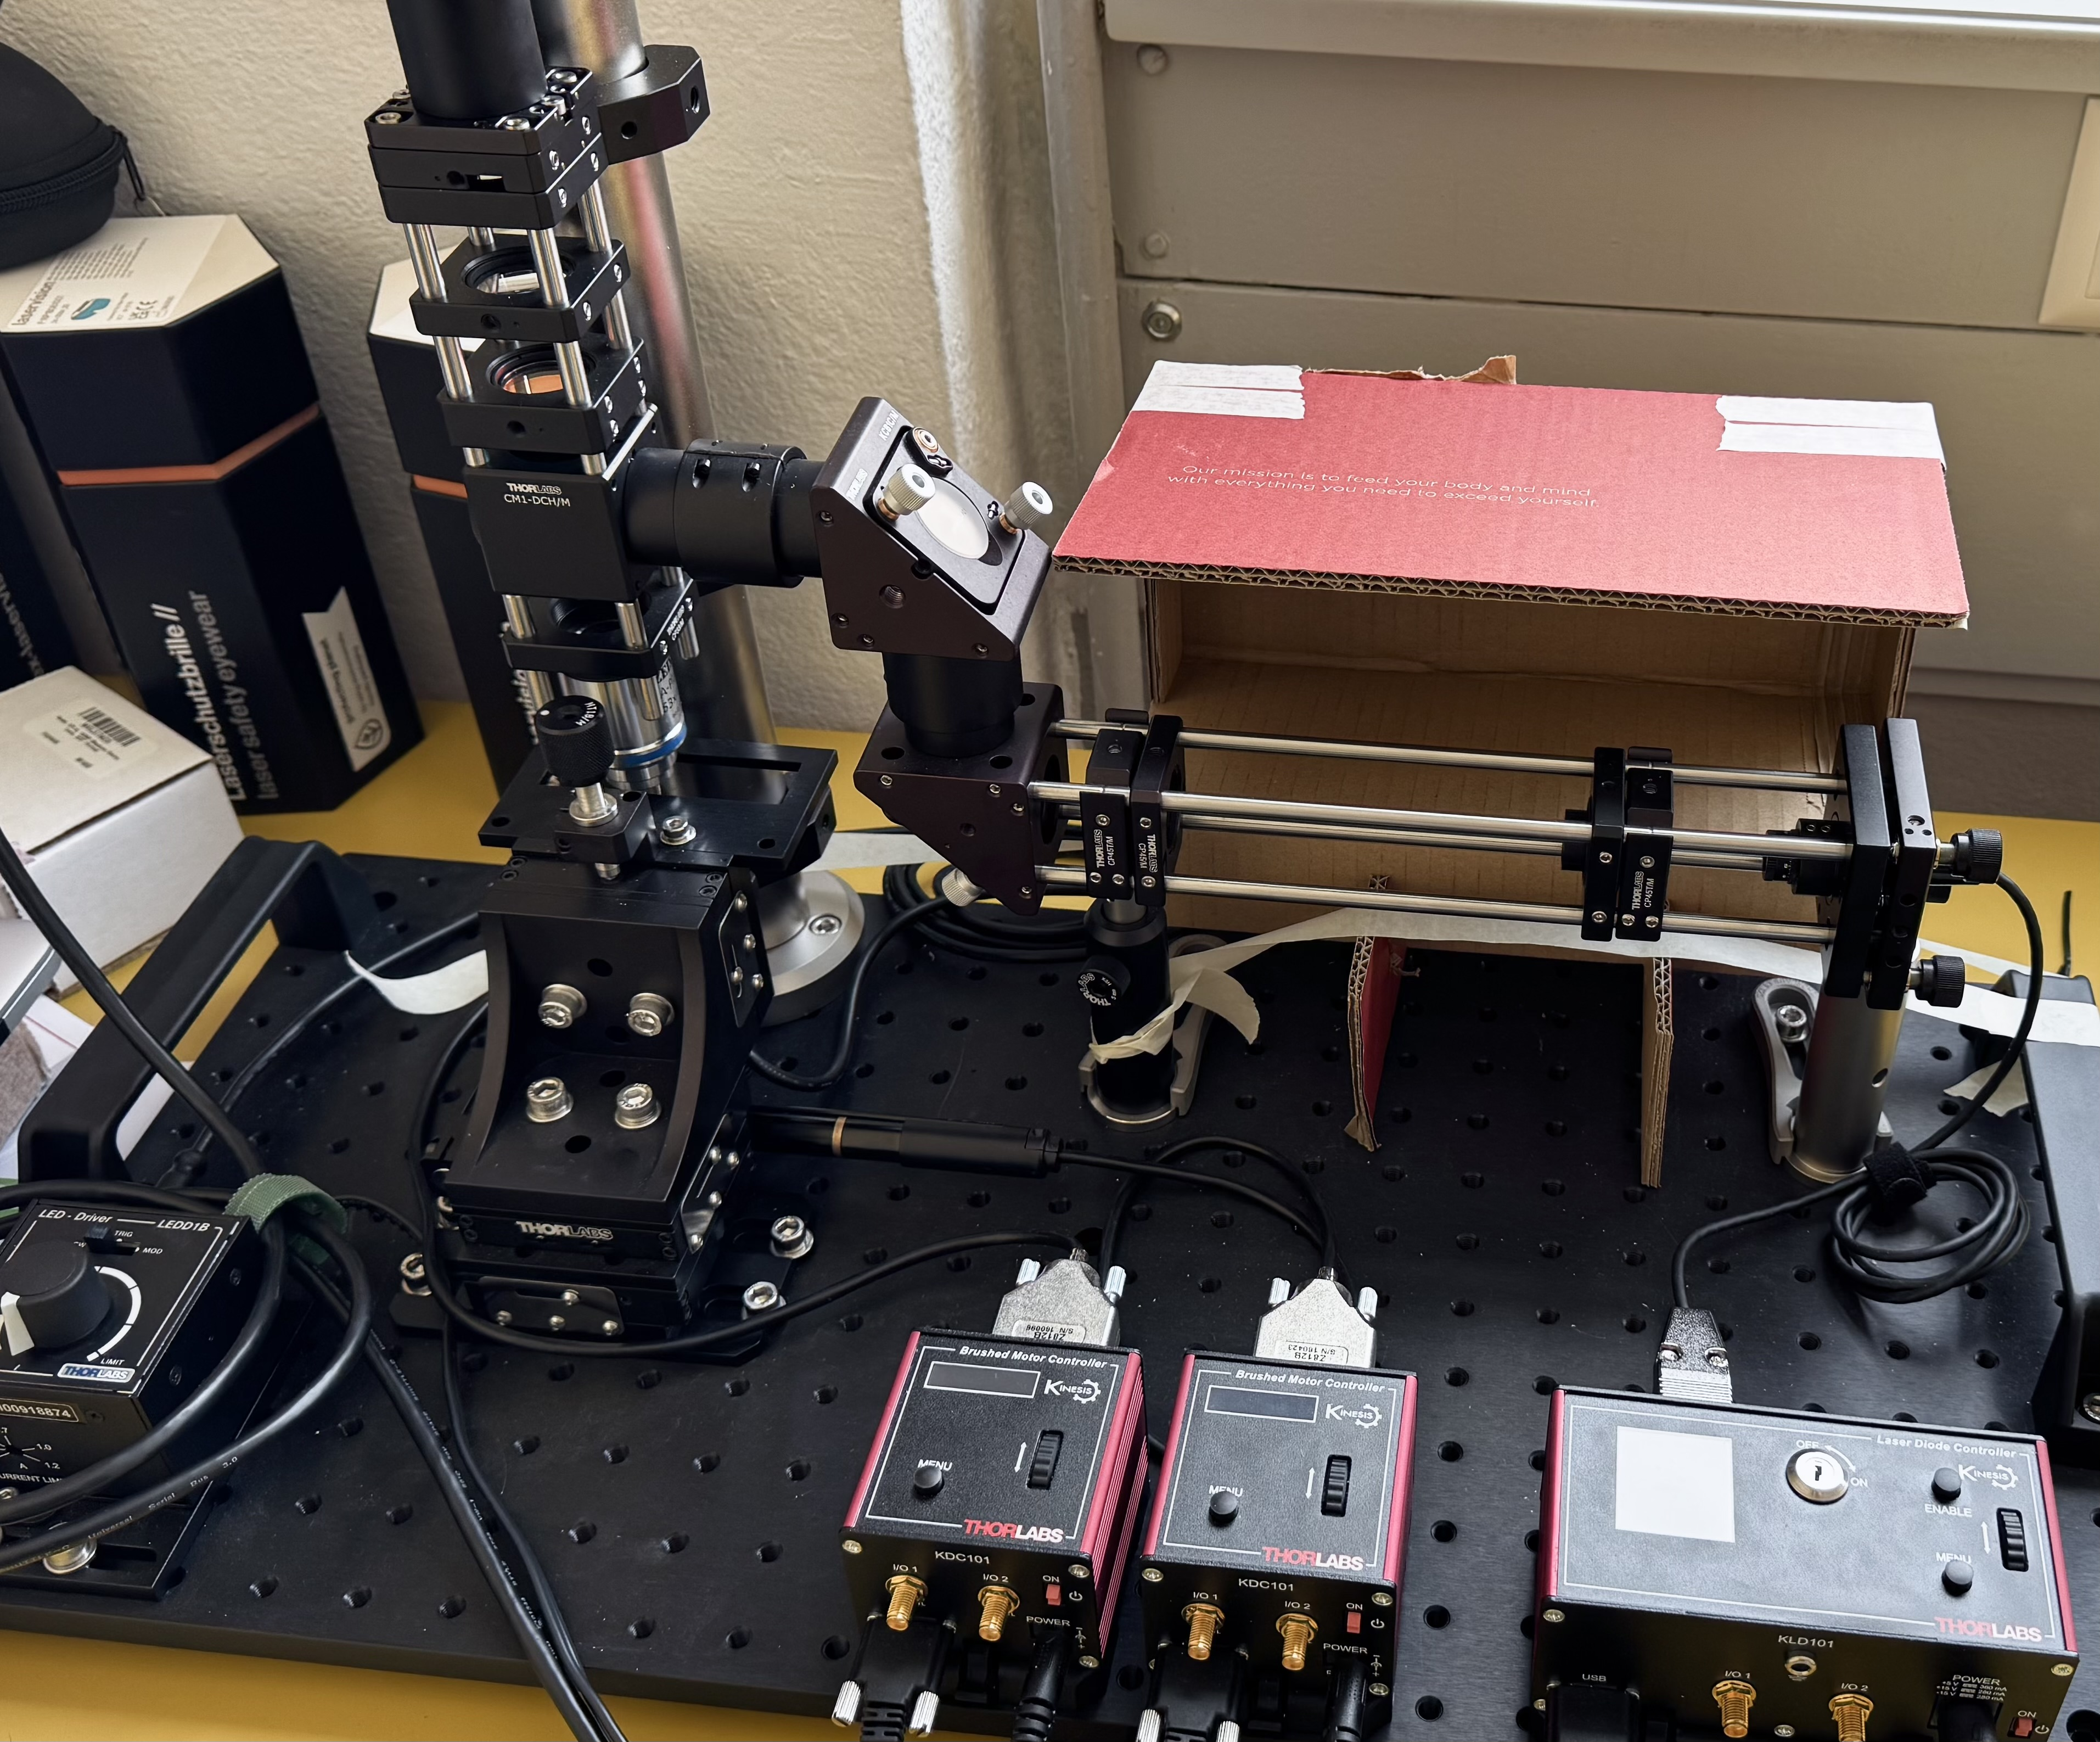
\includegraphics[width=\textwidth]{assets/figures/Protections_laser/Securite_mecanique/Protection_entree_laser/carton_protection_ouvert.jpeg}
        \end{center}
        \captionof{figure}{Prototype en carton, protection ouverte}
        \label{carton_protection_ouverte}
    \end{minipage}
\end{minipage}

\begin{minipage}{\textwidth}
    \subsection{Modélisation de la protection}
    Maintenant que l'idée principale est présente, il faut passer à la modélisation de la protection. Avant cette étape, la représentation en 3D du kit complet a été faite, comme expliqué à la page~\pageref{modelisation_3D} au premier paragraphe. Le 3D du kit permet de pouvoir créer la protection en tenant compte de  toutes les contraintes liés aux autres composants, sans devoir faire des mesures sur le kit réel.

    Pour pouvoir mieux comprendre les choix de conception et les étapes faites pour réaliser la protection, les Figures~\ref{model_3D_ferme}~et~\ref{model_3D_ouvert}, ci-dessous, représente la modélisation complète de la protection ouverte et fermée.

    \begin{minipage}[c]{0.48\textwidth}
        \begin{center}
            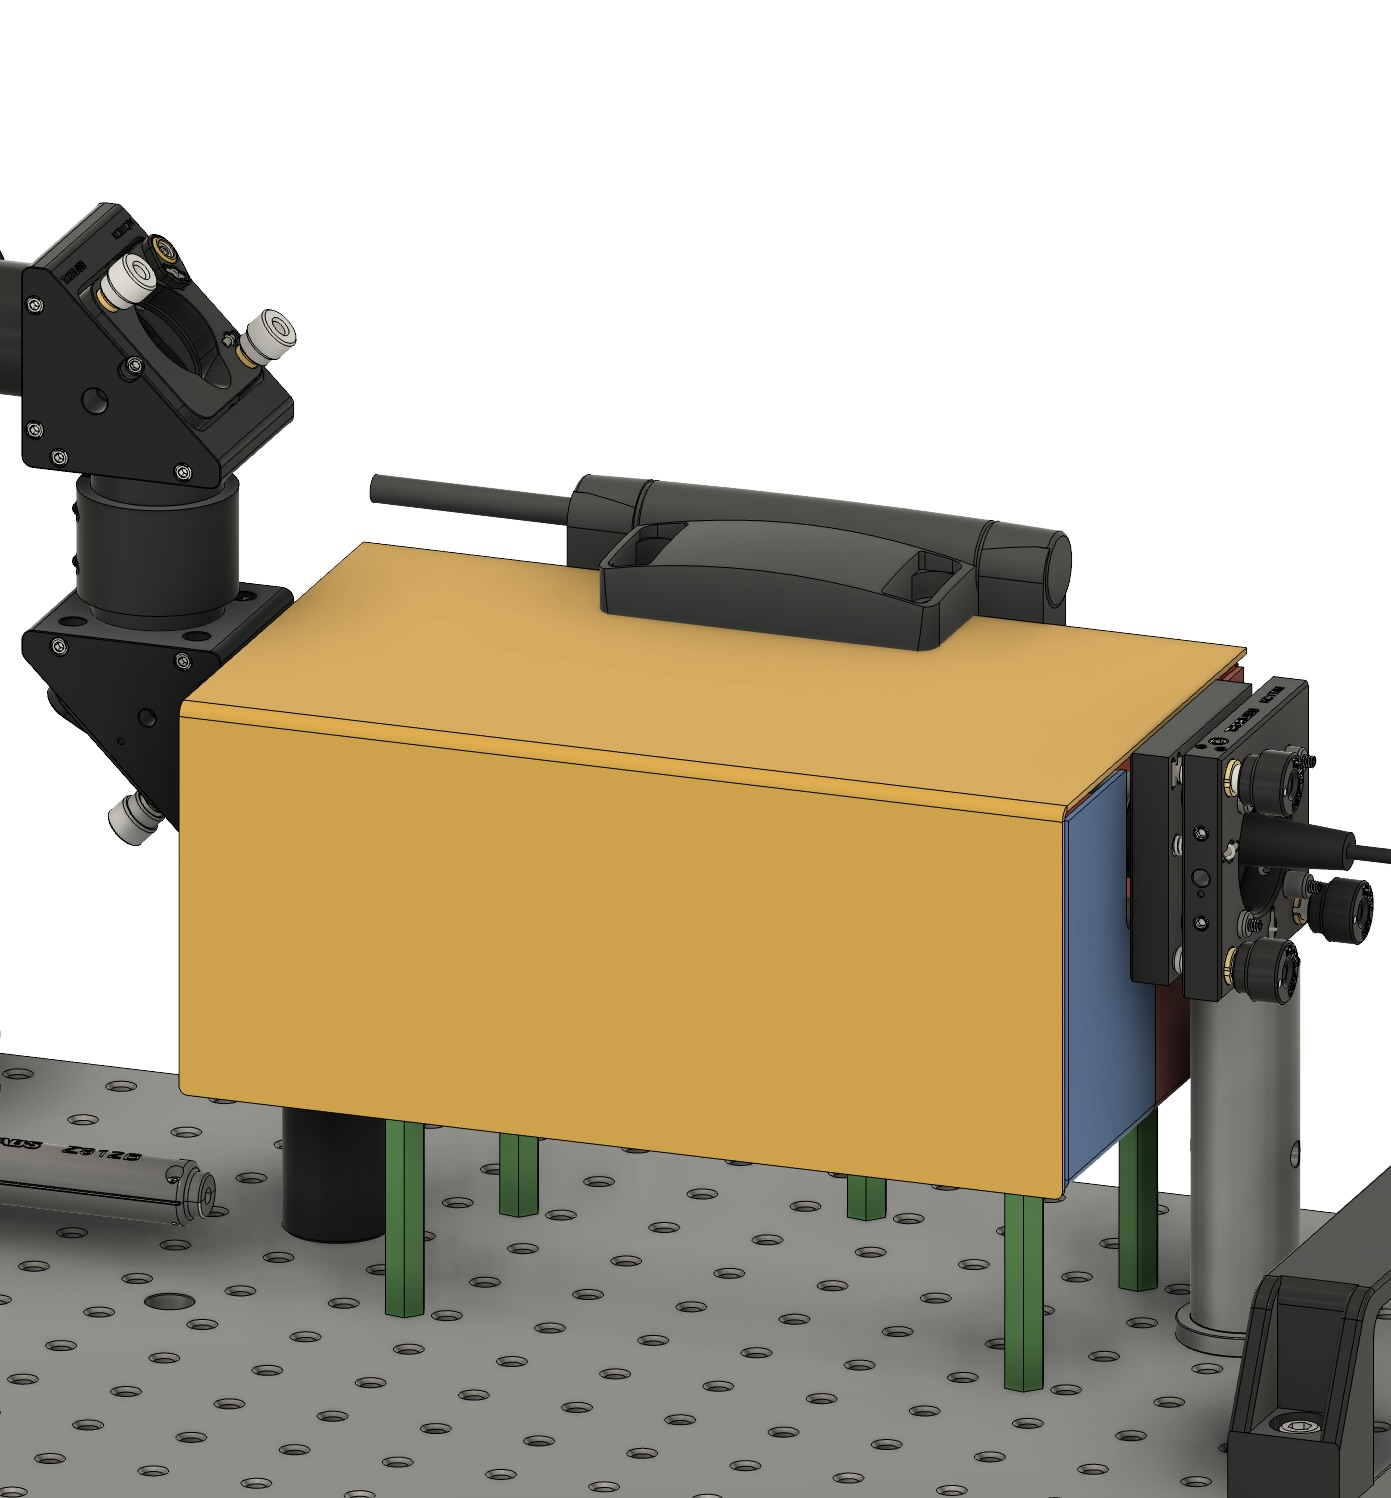
\includegraphics[width=\textwidth]{assets/figures/Protections_laser/Securite_mecanique/Protection_entree_laser/model_3D_ferme.jpeg}
        \end{center}
        \captionof{figure}{Modèle 3D de la protection ouverte}
        \label{model_3D_ferme}
    \end{minipage}\hfill
    \begin{minipage}[c]{0.48\textwidth}
        \begin{center}
            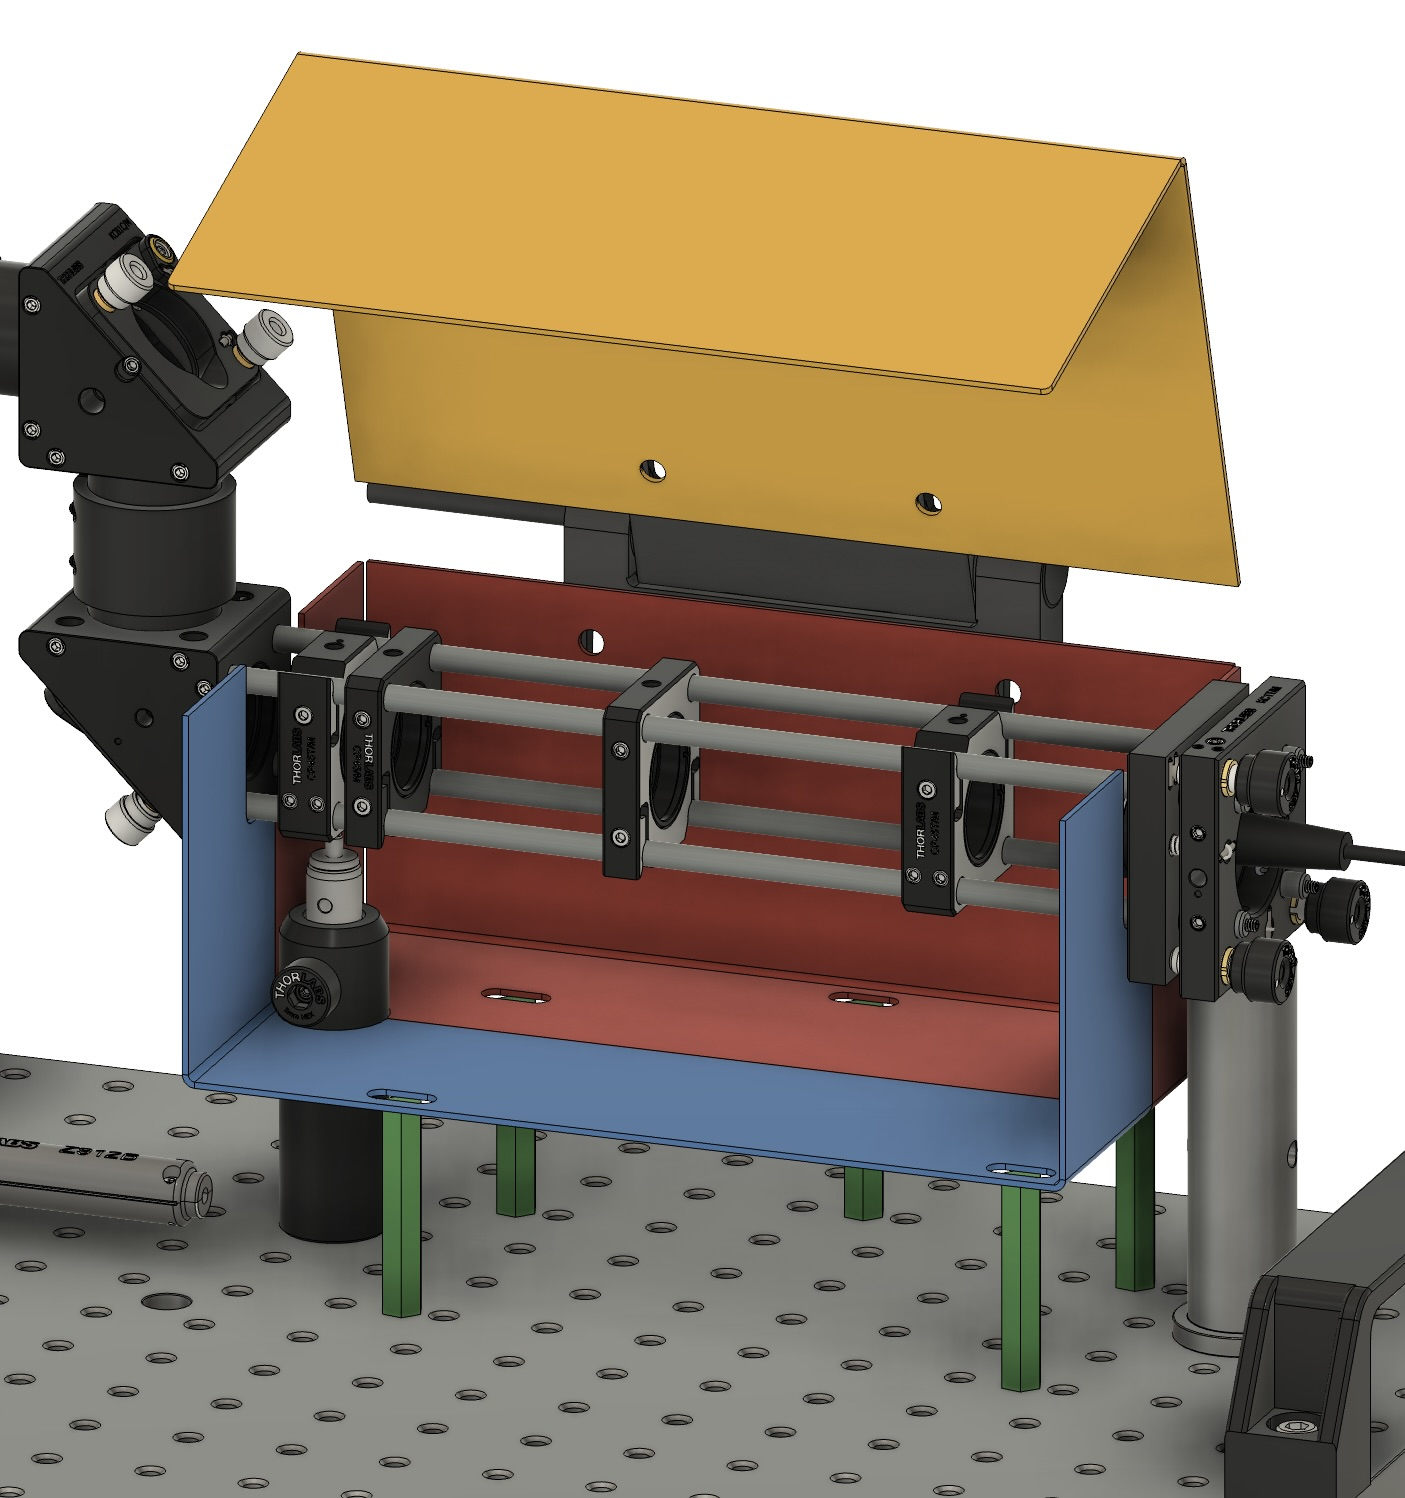
\includegraphics[width=\textwidth]{assets/figures/Protections_laser/Securite_mecanique/Protection_entree_laser/model_3D_ouvert.jpeg}
        \end{center}
        \captionof{figure}{Modèle 3D de la protection fermée}
        \label{model_3D_ouvert}
    \end{minipage}

    % Prompt ChatGPT pour la création du tableau:
    % Explication des pièces modélisées représentées en couleur pour la protection à l'entrée du laser
    % \begin{itemize}
    %     \item \textcolor[RGB]{88, 122, 163}{En bleu}, le capot inférieur avant.
    %     \item \textcolor[RGB]{170, 80, 70}{En rouge}, le capot inférieur arrière.
    %     \item \textcolor[RGB]{233, 173, 56}{En jaune}, le capot supérieur.
    %     \item \textcolor[RGB]{100, 100, 100}{En gris foncé}, la charnière qui relie le capot inférieur arrière et le capot supérieur.
    %     \item \textcolor[RGB]{70, 170, 70}{En vert}, les entretoises qui supportent les capots inférieurs avant et arrière.
    % \end{itemize}
    % fais en plutot un tableau en latex

    \begin{table}[H]
        \centering
        \begin{tabular}{|c|l|}
            \hline
            \textbf{Couleur}                           & \textbf{Nom de la pièce}                             \\
            \hline
            \textcolor[RGB]{88, 122, 163}{Bleu}        & Capot inférieur avant                                \\
            \textcolor[RGB]{170, 80, 70}{Rouge}        & Capot inférieur arrière                              \\
            \textcolor[RGB]{233, 173, 56}{Jaune}       & Capot supérieur                                      \\
            \textcolor[RGB]{100, 100, 100}{Gris foncé} & Charnière reliant la partie inférieure et supérieure \\
            \textcolor[RGB]{70, 170, 70}{Vert}         & Entretoises supportant les capots inférieurs         \\
            \hline
        \end{tabular}
        \caption{Nomenclature des pièces modélisées avec code couleur pour la protection à l'entrée du laser. \cite{chatgptTableProtectionEntreeLaser}}
        \label{tab:nomenclature_pieces_laser}
    \end{table}
\end{minipage}
\subsubsection{Contraintes rencontrées}

\begin{minipage}[c]{0.4\textwidth}
    La première contrainte a été cet axe noir vertical que l'on voit par la flèche noir sur la Figure~\ref{contrainte_axe_vertical} qui passent à travers les deux capots inférieurs.

    La solution s'est résumée à séparer le capot inférieur en deux, aidant à assembler facilement sans devoir démonter des pièces du kit original.
\end{minipage}\hfill
\begin{minipage}[c]{0.58\textwidth}
    \begin{center}
        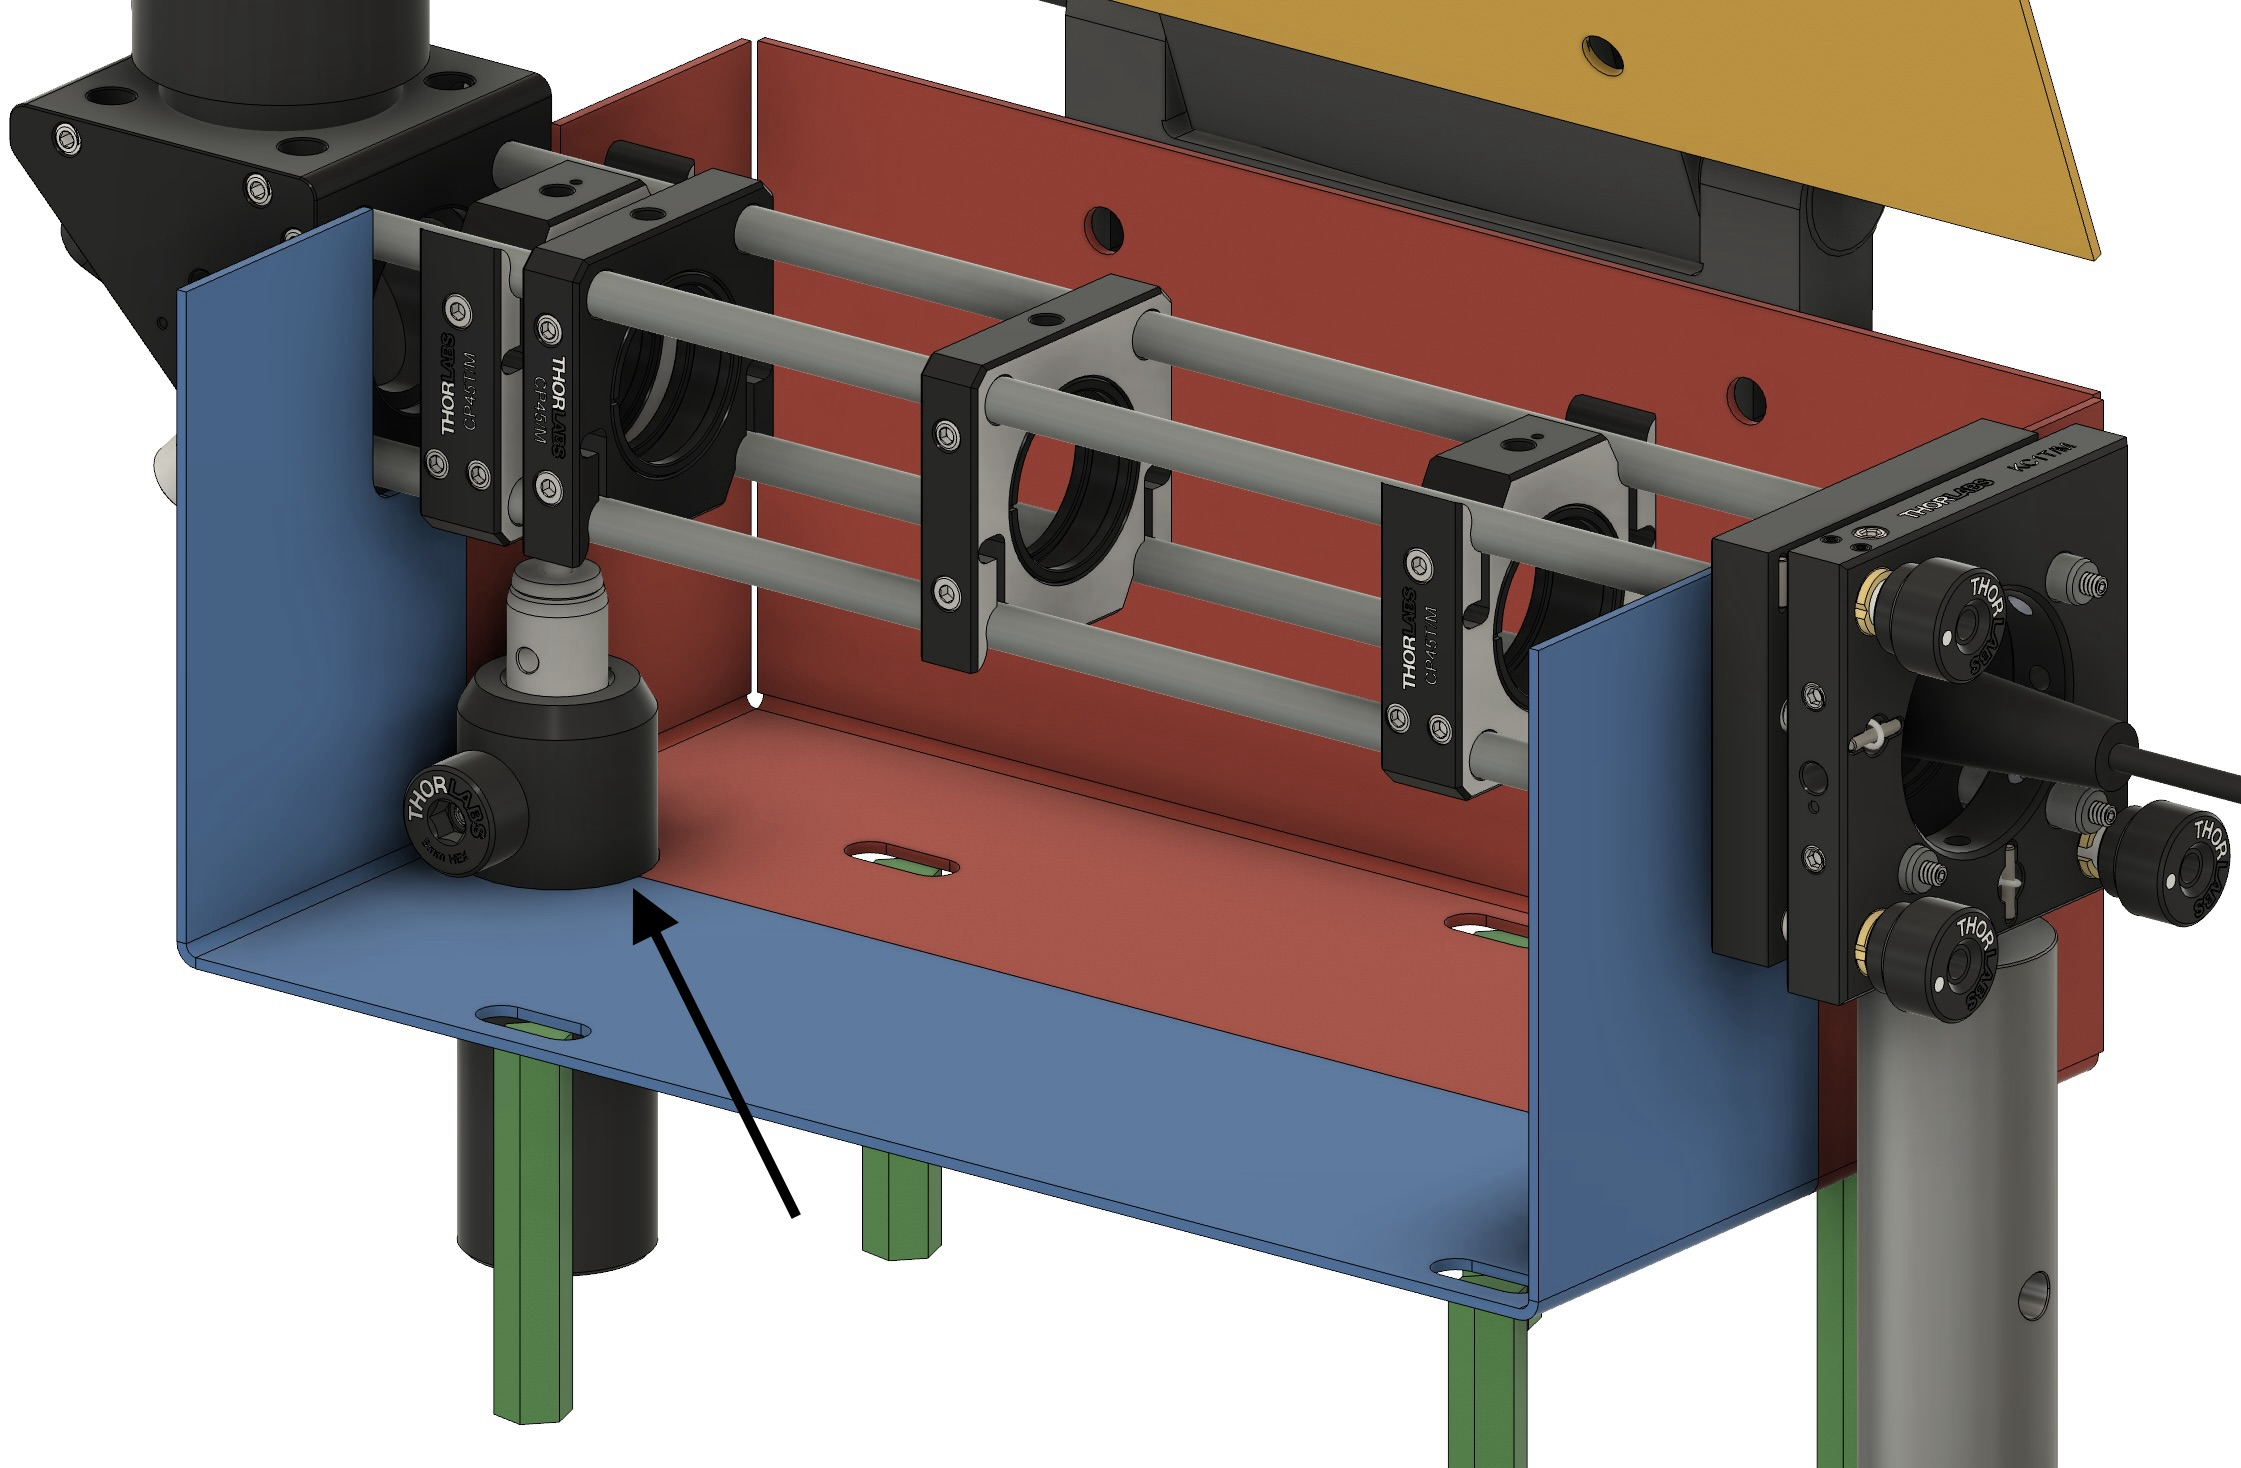
\includegraphics[width=\textwidth]{assets/figures/Protections_laser/Securite_mecanique/Protection_entree_laser/contrainte_axe_vertical.jpeg}
    \end{center}
    \captionof{figure}{Vue en perspective cavalière: Axe vertical traversant les protections inférieures}
    \label{contrainte_axe_vertical}
\end{minipage}

\begin{minipage}[c]{0.4\textwidth}
    Une seconde contrainte a été cette vis de réglage indiquée par la flèche noir sur la Figure~\ref{contrainte_vis}. Elle se situe dans la course du capot supérieur.

    La solution retenue a été de s'assurer que toutes les protections, dans le plan horizontal, ne dépassent pas la largeur de la vis. Cette contrainte en entraîne une autre, qui sera détaillée ensuite.
\end{minipage}\hfill
\begin{minipage}[c]{0.58\textwidth}
    \begin{center}
        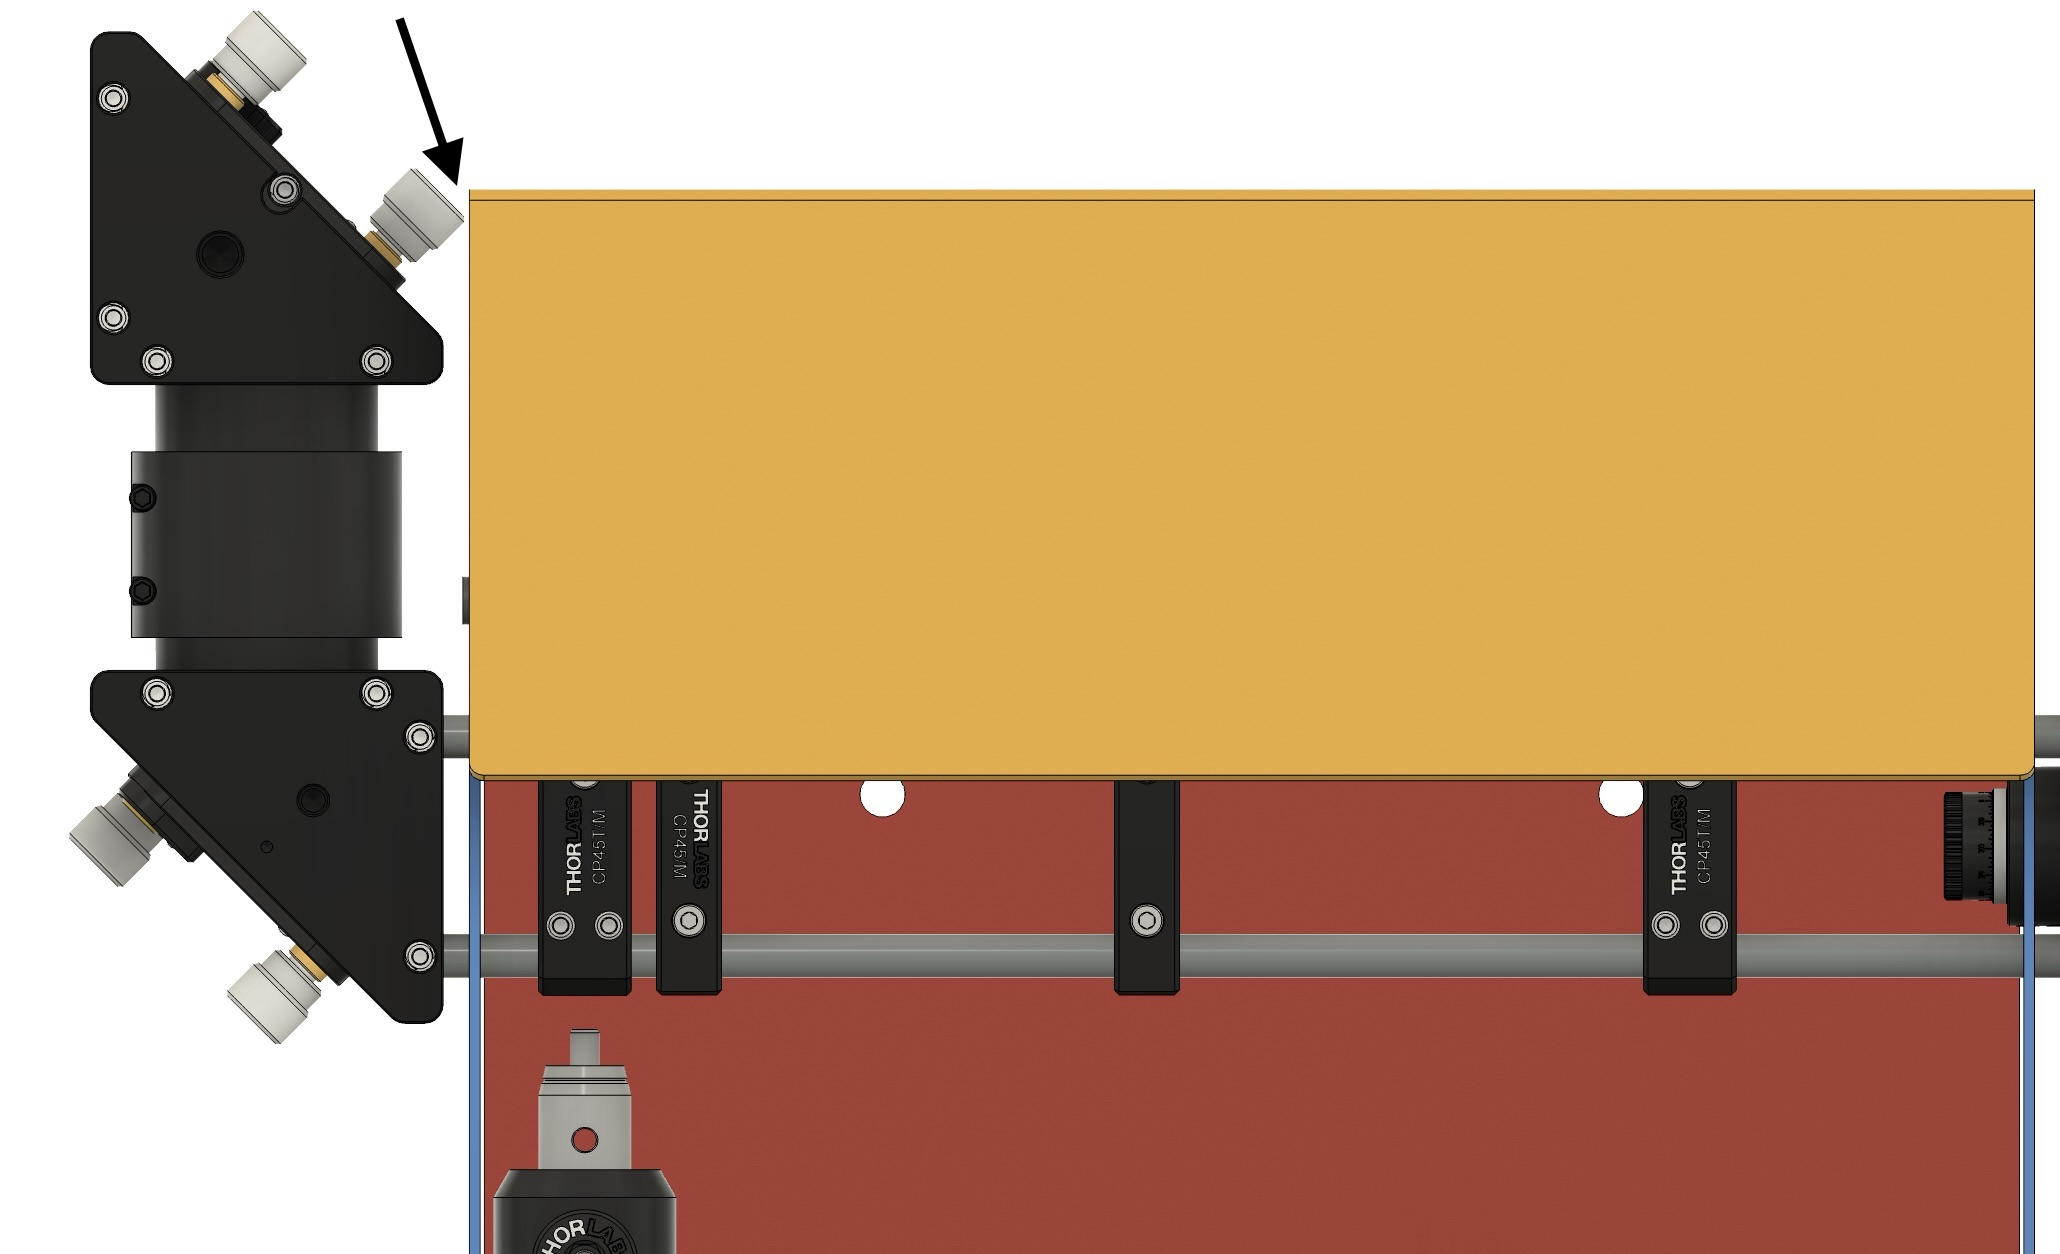
\includegraphics[width=\textwidth]{assets/figures/Protections_laser/Securite_mecanique/Protection_entree_laser/contrainte_vis.jpeg}
    \end{center}
    \captionof{figure}{Vue de face: Vis de réglage dans la course du capot supérieur}
    \label{contrainte_vis}
\end{minipage}

\begin{minipage}[c]{0.5\textwidth}
    En effet, l'obligation de réduire la taille des protections, cela crée un vide pouvant laisser passer les rayons du laser. Les traits manuscrits en rouge sur la Figure~\ref{contrainte_passage_laser_cage} représentent les fuites potentielles du laser. Ce phénomène apparaît également à droite de la protection.

    La solution apportée a été d'ajouter un joint en mousse souple entourant les quatres axes formant la cage. Les protections s'appuyent sur les joints et comblent dorénavant les vides. Les détails en photo pour cette solution sont montrés sur la Figure~\ref{montage_bois} à la section~\ref{prototype_bois}.
\end{minipage}\hfill
\begin{minipage}[c]{0.48\textwidth}
    \begin{center}
        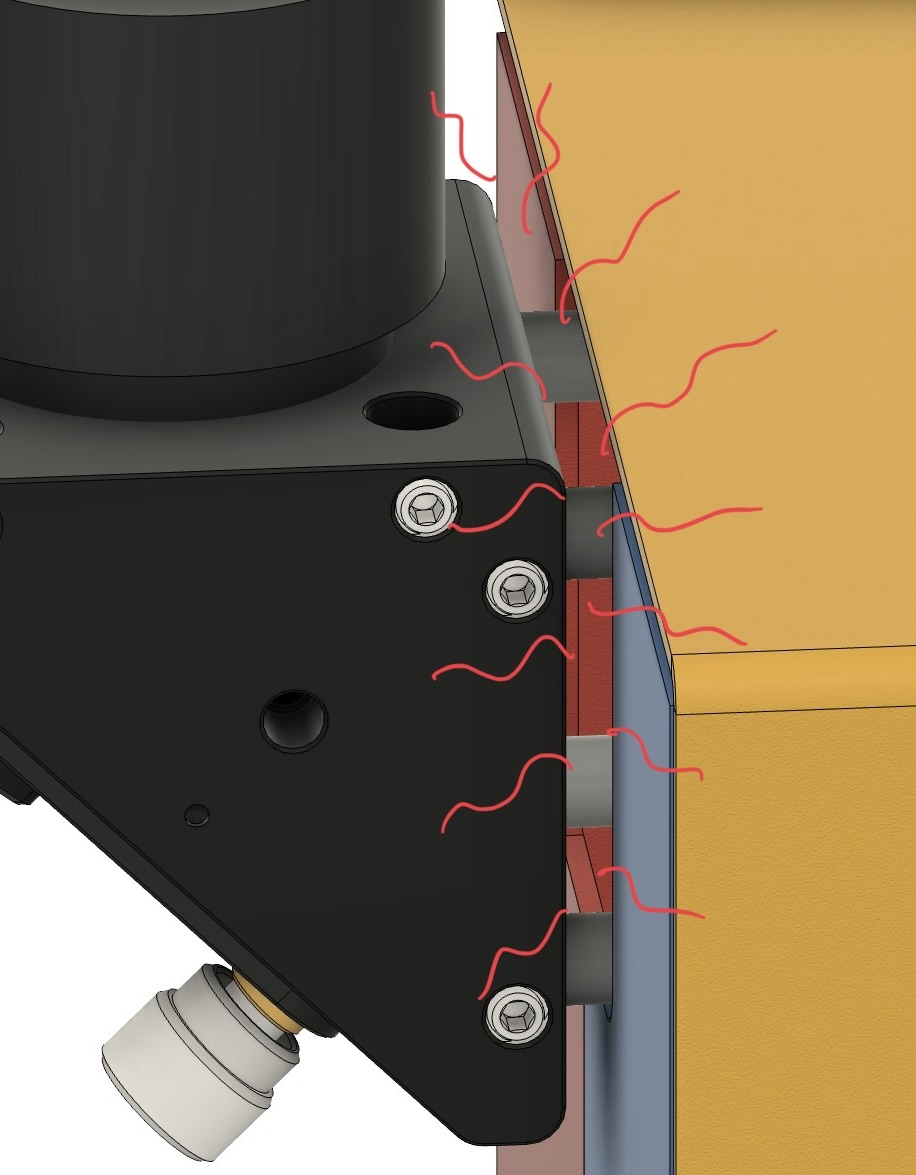
\includegraphics[width=0.9\textwidth]{assets/figures/Protections_laser/Securite_mecanique/Protection_entree_laser/contrainte_passage_laser_cage.jpeg}
    \end{center}
    \captionof{figure}{Vue en perspective cavalière: Fuites potentielles des rayons du laser pour les capots inférieurs}
    \label{contrainte_passage_laser_cage}
\end{minipage}

\begin{minipage}[c]{0.6\textwidth}
    La contrainte expliquée ici, similaire à la précédente, vient contrer les fuites possibles du laser. Cependant, cette fois, c'est pour la protection supérieure. En effet, lorsque le capot est fermé, il y a un risque d'avoir des espaces fins où la lumière du faisceau peut s'échapper.

    La solution va également être la pose d'un joint, cette fois à l'intérieur du capot supérieur sur tout son contour. Ainsi, lorsque la protection est fermée, le joint comblera les vides. La modélisation ci-contre, voir la Figure~\ref{contrainte_passage_laser_capot}, montre qu'un espace entre la partie inférieure est supérieur de la protection a volontairement été créer afin de laisser de la place pour le joint.

    On peut apercevoir plus loin sur la Figure~\ref{montage_alu_ouvert} à la section~\ref{montage_final} la pose du joint.
\end{minipage}\hfill
\begin{minipage}[c]{0.38\textwidth}
    \begin{center}
        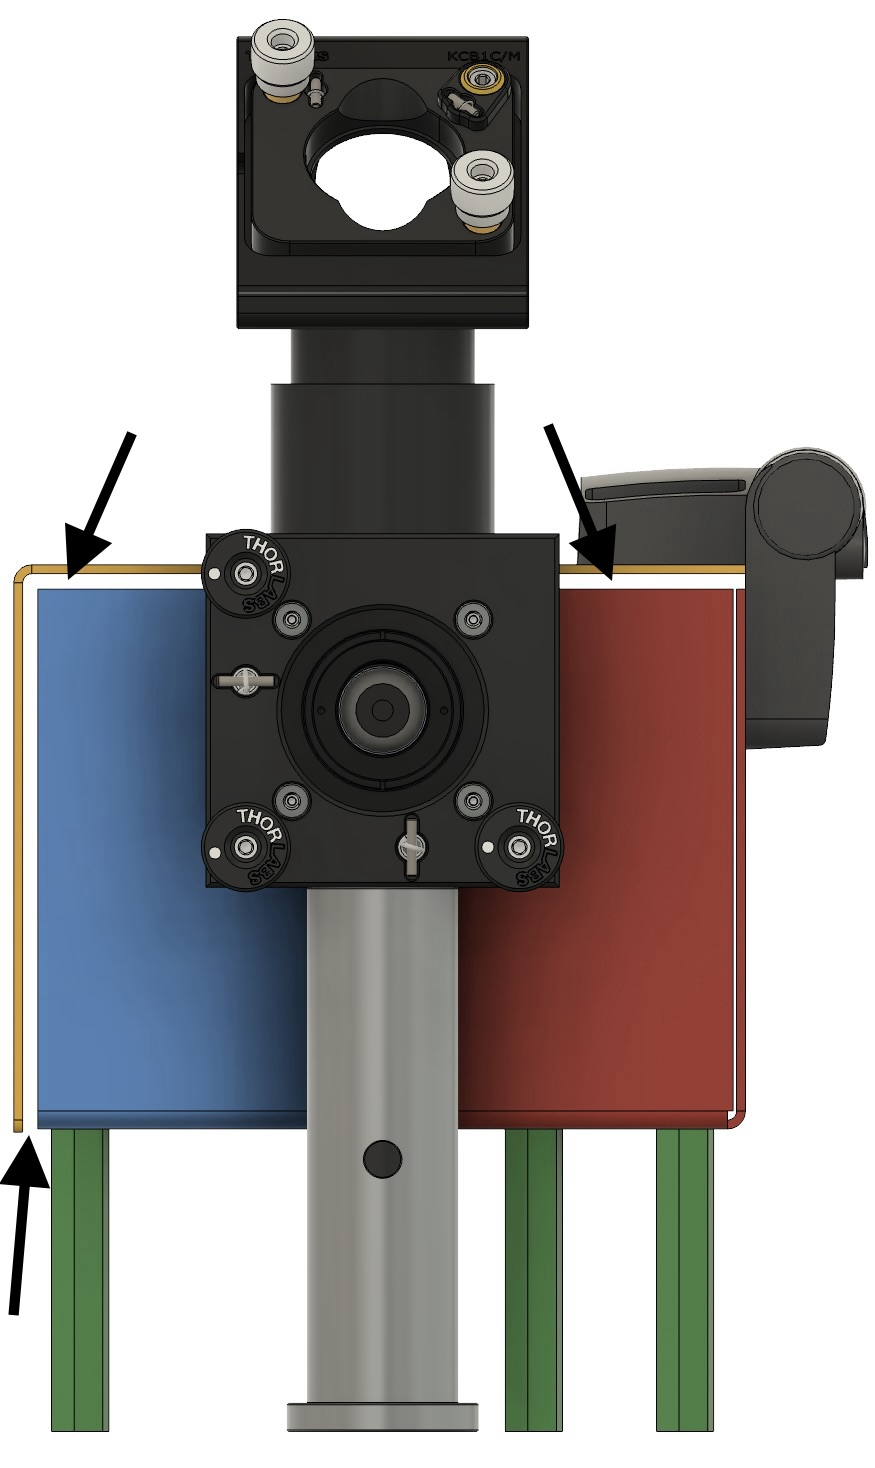
\includegraphics[width=0.8\textwidth]{assets/figures/Protections_laser/Securite_mecanique/Protection_entree_laser/contrainte_passage_laser_capot.jpeg}
    \end{center}
    \captionof{figure}{Vue de droite: Fuites potentielles des rayons du laser pour le capot supérieur}
    \label{contrainte_passage_laser_capot}
\end{minipage}

\begin{minipage}{\textwidth}
    La dernière problématique est: comment fixer les protections au kit ? Comme la plaque de montage en aluminium, où sont fixés tous les composants du kit, contient des taraudages M6 sur toute sa surface, il est facile de trouver des encrages de fixation.

    La solution trouvée, illustrée ci-dessous, est d'utiliser des entretoises; deux pour fixer le capot inférieur avant et trois pour le capot inférieur arrière. Ce dernier en contient plus, car subit plus de contraintes mécaniques. L'addition de la masse du capot inférieur arrière, de la charnière et du capot supérieur engendre un poids conséquent. Évidemment, il a fallu prêter attention aux composants déjà positionnés et choisir judicieusement les emplacements des entretoises.

    Une entretoise hexagonale mesure 50~mm de hauteur, 8~mm de largeur et un taraudage M6 à chaque extrémité.

    Pour avoir une marge de sécurité, des oblongs ont été réalisés sur les tôles afin de faciliter leur fixation.
    \vspace{1em}
    \begin{center}
        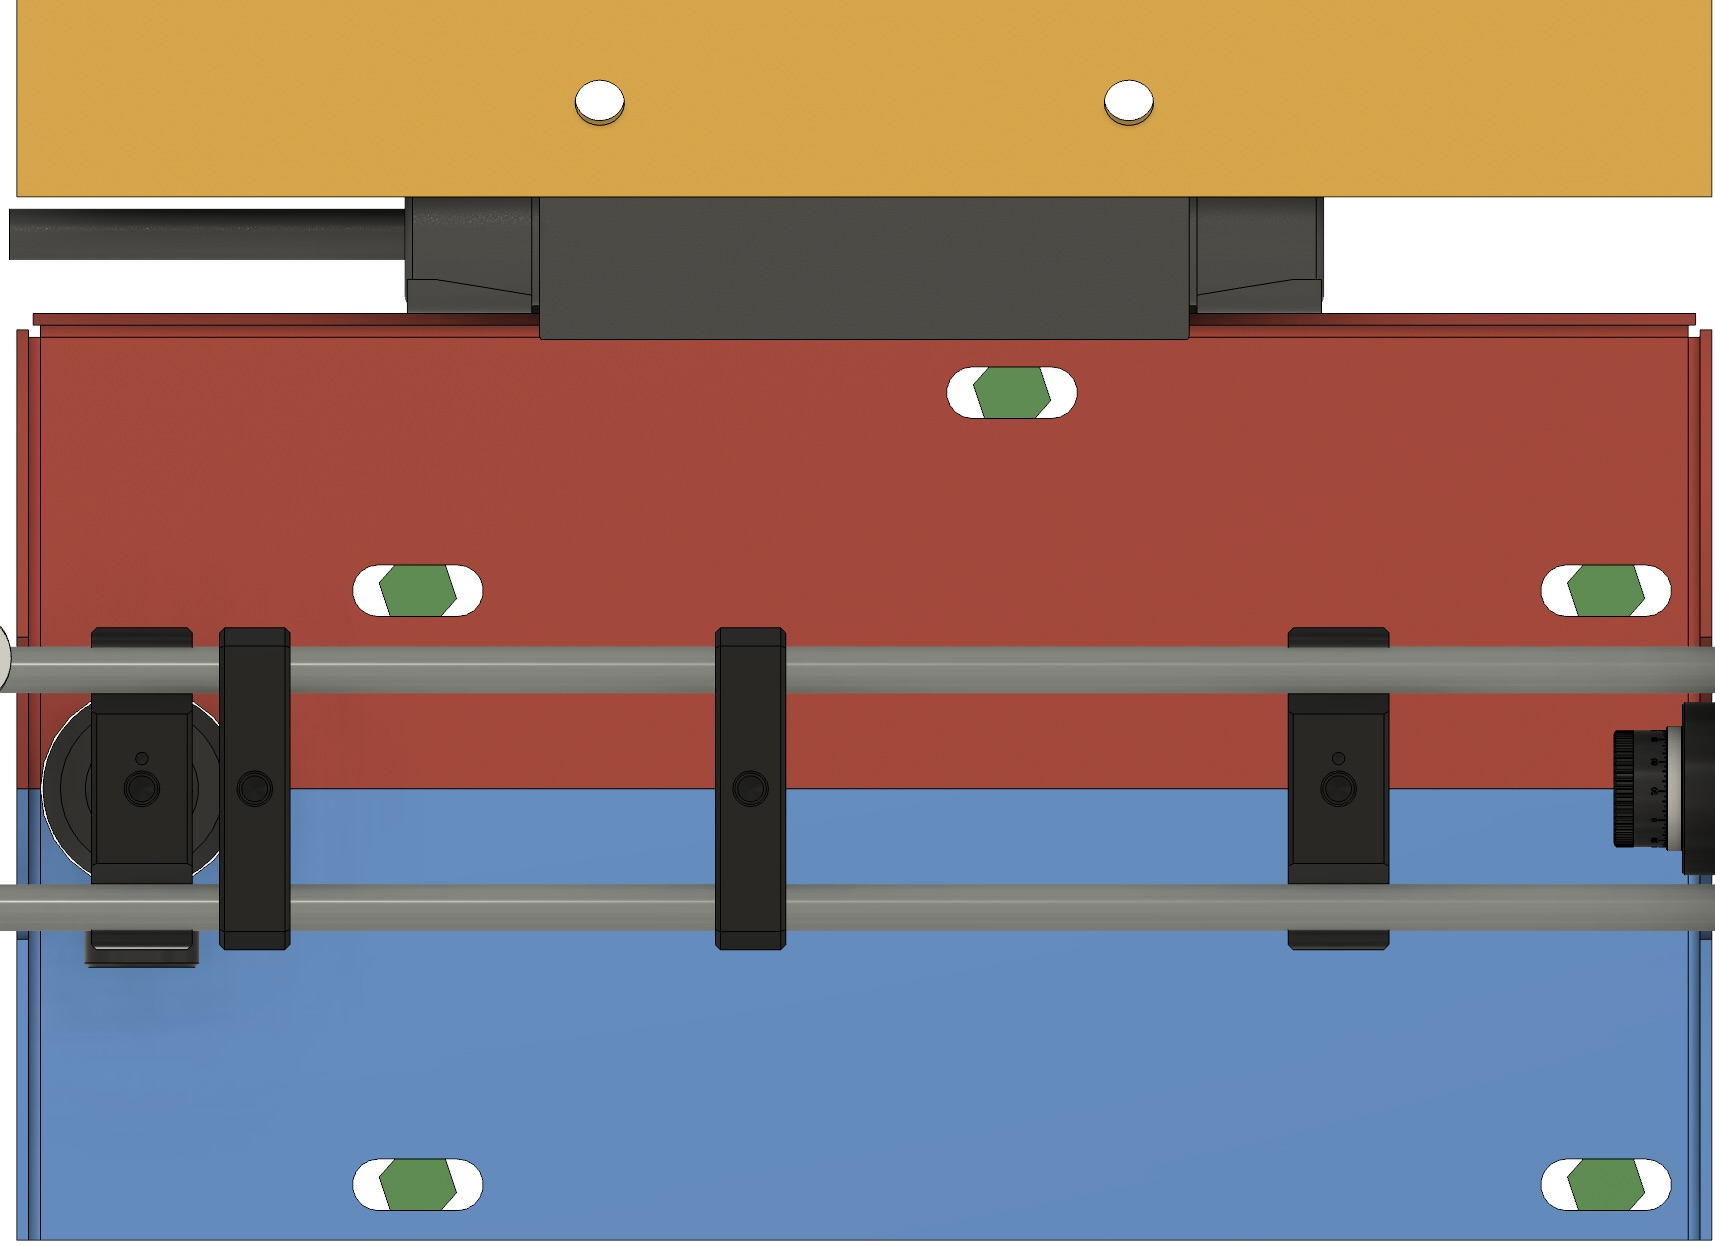
\includegraphics[width=0.6\textwidth]{assets/figures/Protections_laser/Securite_mecanique/Protection_entree_laser/contrainte_entretoises.jpeg}
    \end{center}
    \captionof{figure}{Vue de dessus: cinq entretoises pour fixer les capots au kit}
    \label{contrainte_entretoises}
\end{minipage}

\subsection{Mise en plan des pièces modélisées}
La modélisation terminée, il faut passer à la réalisation des dessins techniques pour la production des pièces. Une discussion préalable avec le responsable M. Ottonin, de l'atelier mécanique sur le site de Cheseaux, a eu lieu afin de parler du projet. Au cours de cet entretien, le matériau ainsi que l'épaisseur des différentes pièces a été choisi. Pour un usinage facile, le choix s'est porté sur l'aluminium avec une épaisseur de 1.5~mm. Les trois mises en plan se retrouvent au chapitre des annexes \ref{chapter:annexes}, sur les Figures~\ref{mise_en_plan_capot_avant},~\ref{mise_en_plan_capot_arriere}~et~\ref{mise_en_plan_capot_superieur}.






\begin{minipage}[c]{0.48\textwidth}
    \subsection{Réalisation d'un prototype en bois} \label{prototype_bois}
    Une fois les mises en plan faites, j'ai réalisé les trois pièces en MDF d'épaisseur 3~mm acheté chez Jumbo \cite{mdfJumbo}, afin d'être convaincu de la dimension des pièces.

    Pour travailler de manière efficace, j'ai imprimé les dessins techniques à l'échelle~\texttt{1:1}, puis je les ai collés sur les panneaux en bois. Pour finir, j'ai découpé les pièces au cutter. La Figure~\ref{decoupe_bois} illustre ces propos.
    \vspace{1em}
\end{minipage}\hfill
\begin{minipage}[c]{0.48\textwidth}
    \begin{figure}[H]
        \centering
        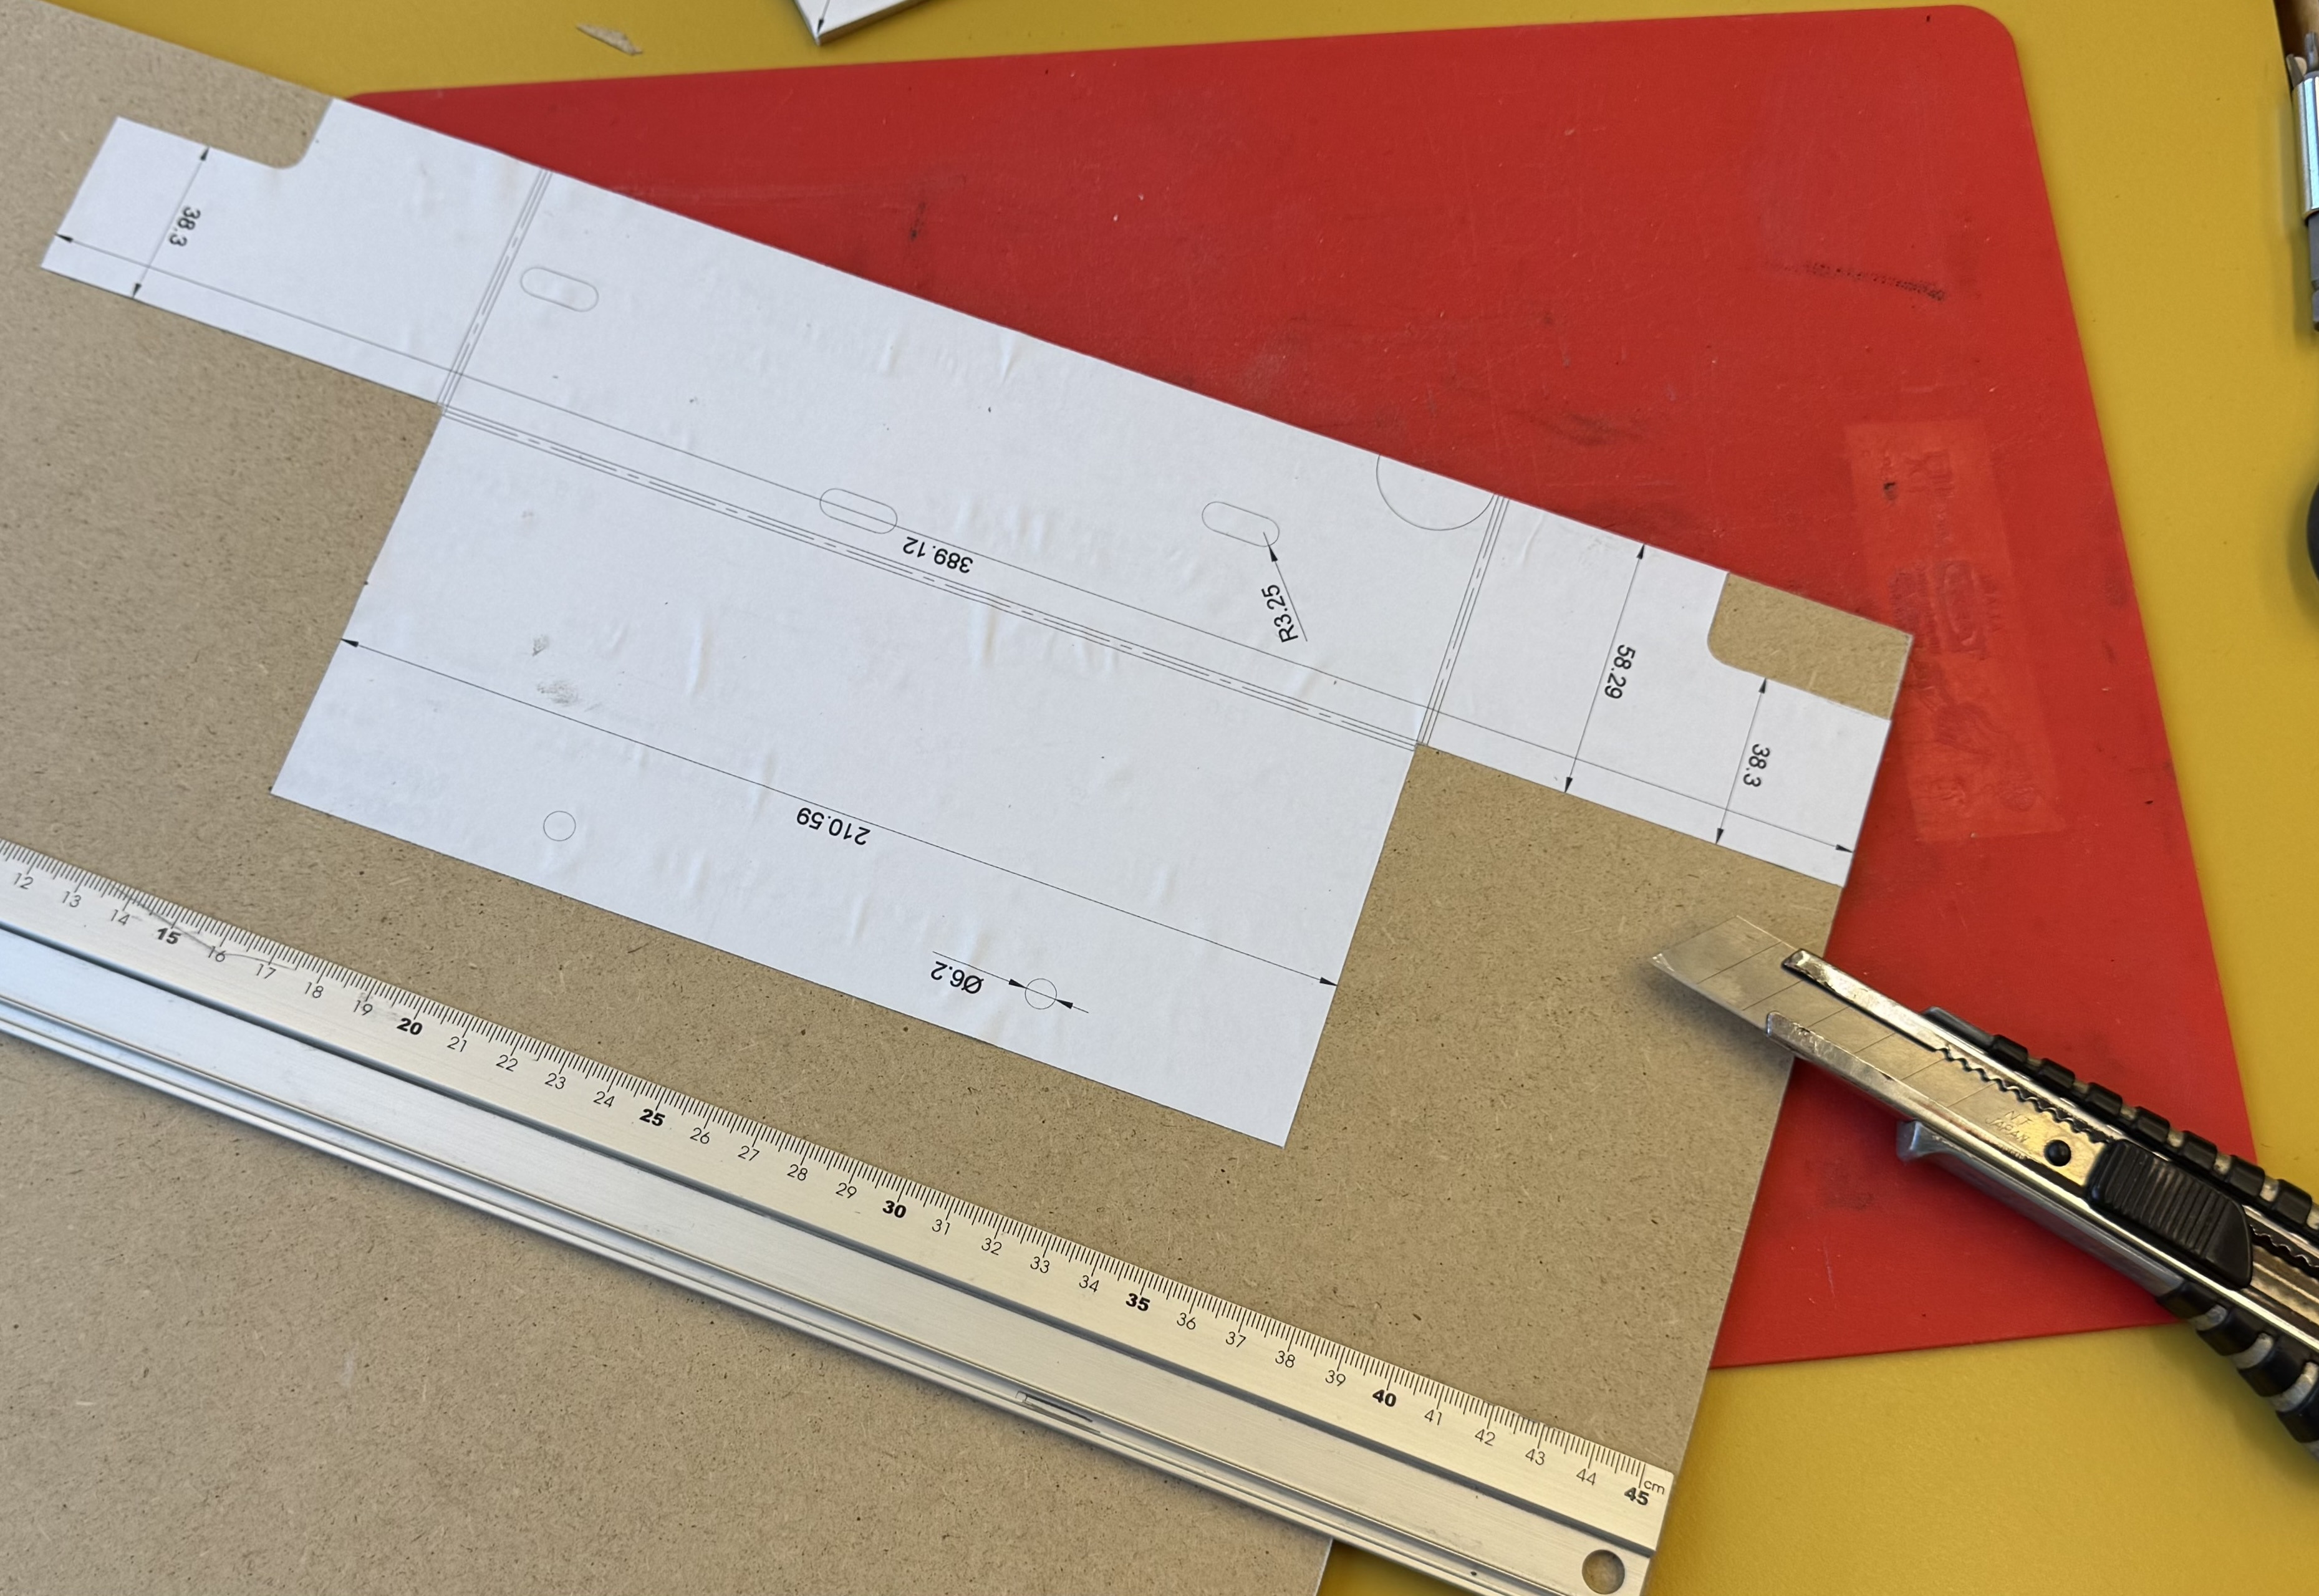
\includegraphics[width=\textwidth]{assets/figures/Protections_laser/Securite_mecanique/Protection_entree_laser/decoupe_bois.jpeg}
        \captionof{figure}{Découpe des protections en bois à l'aide des plans imprimés}
        \label{decoupe_bois}
    \end{figure}
\end{minipage}

\begin{minipage}{\textwidth}
    Pour tenir les différents pliages, des carelets en bois ont été fixés, montrés par les flèches noires sur la Figure~\ref{montage_bois}.

    La flèche \textcolor{red}{rouge} désigne le joint qui empêche les rayons du laser de passer outre la protection. Le joint a une épaisseur de 3~mm au repos.
    \vspace{1em}
    \begin{center}
        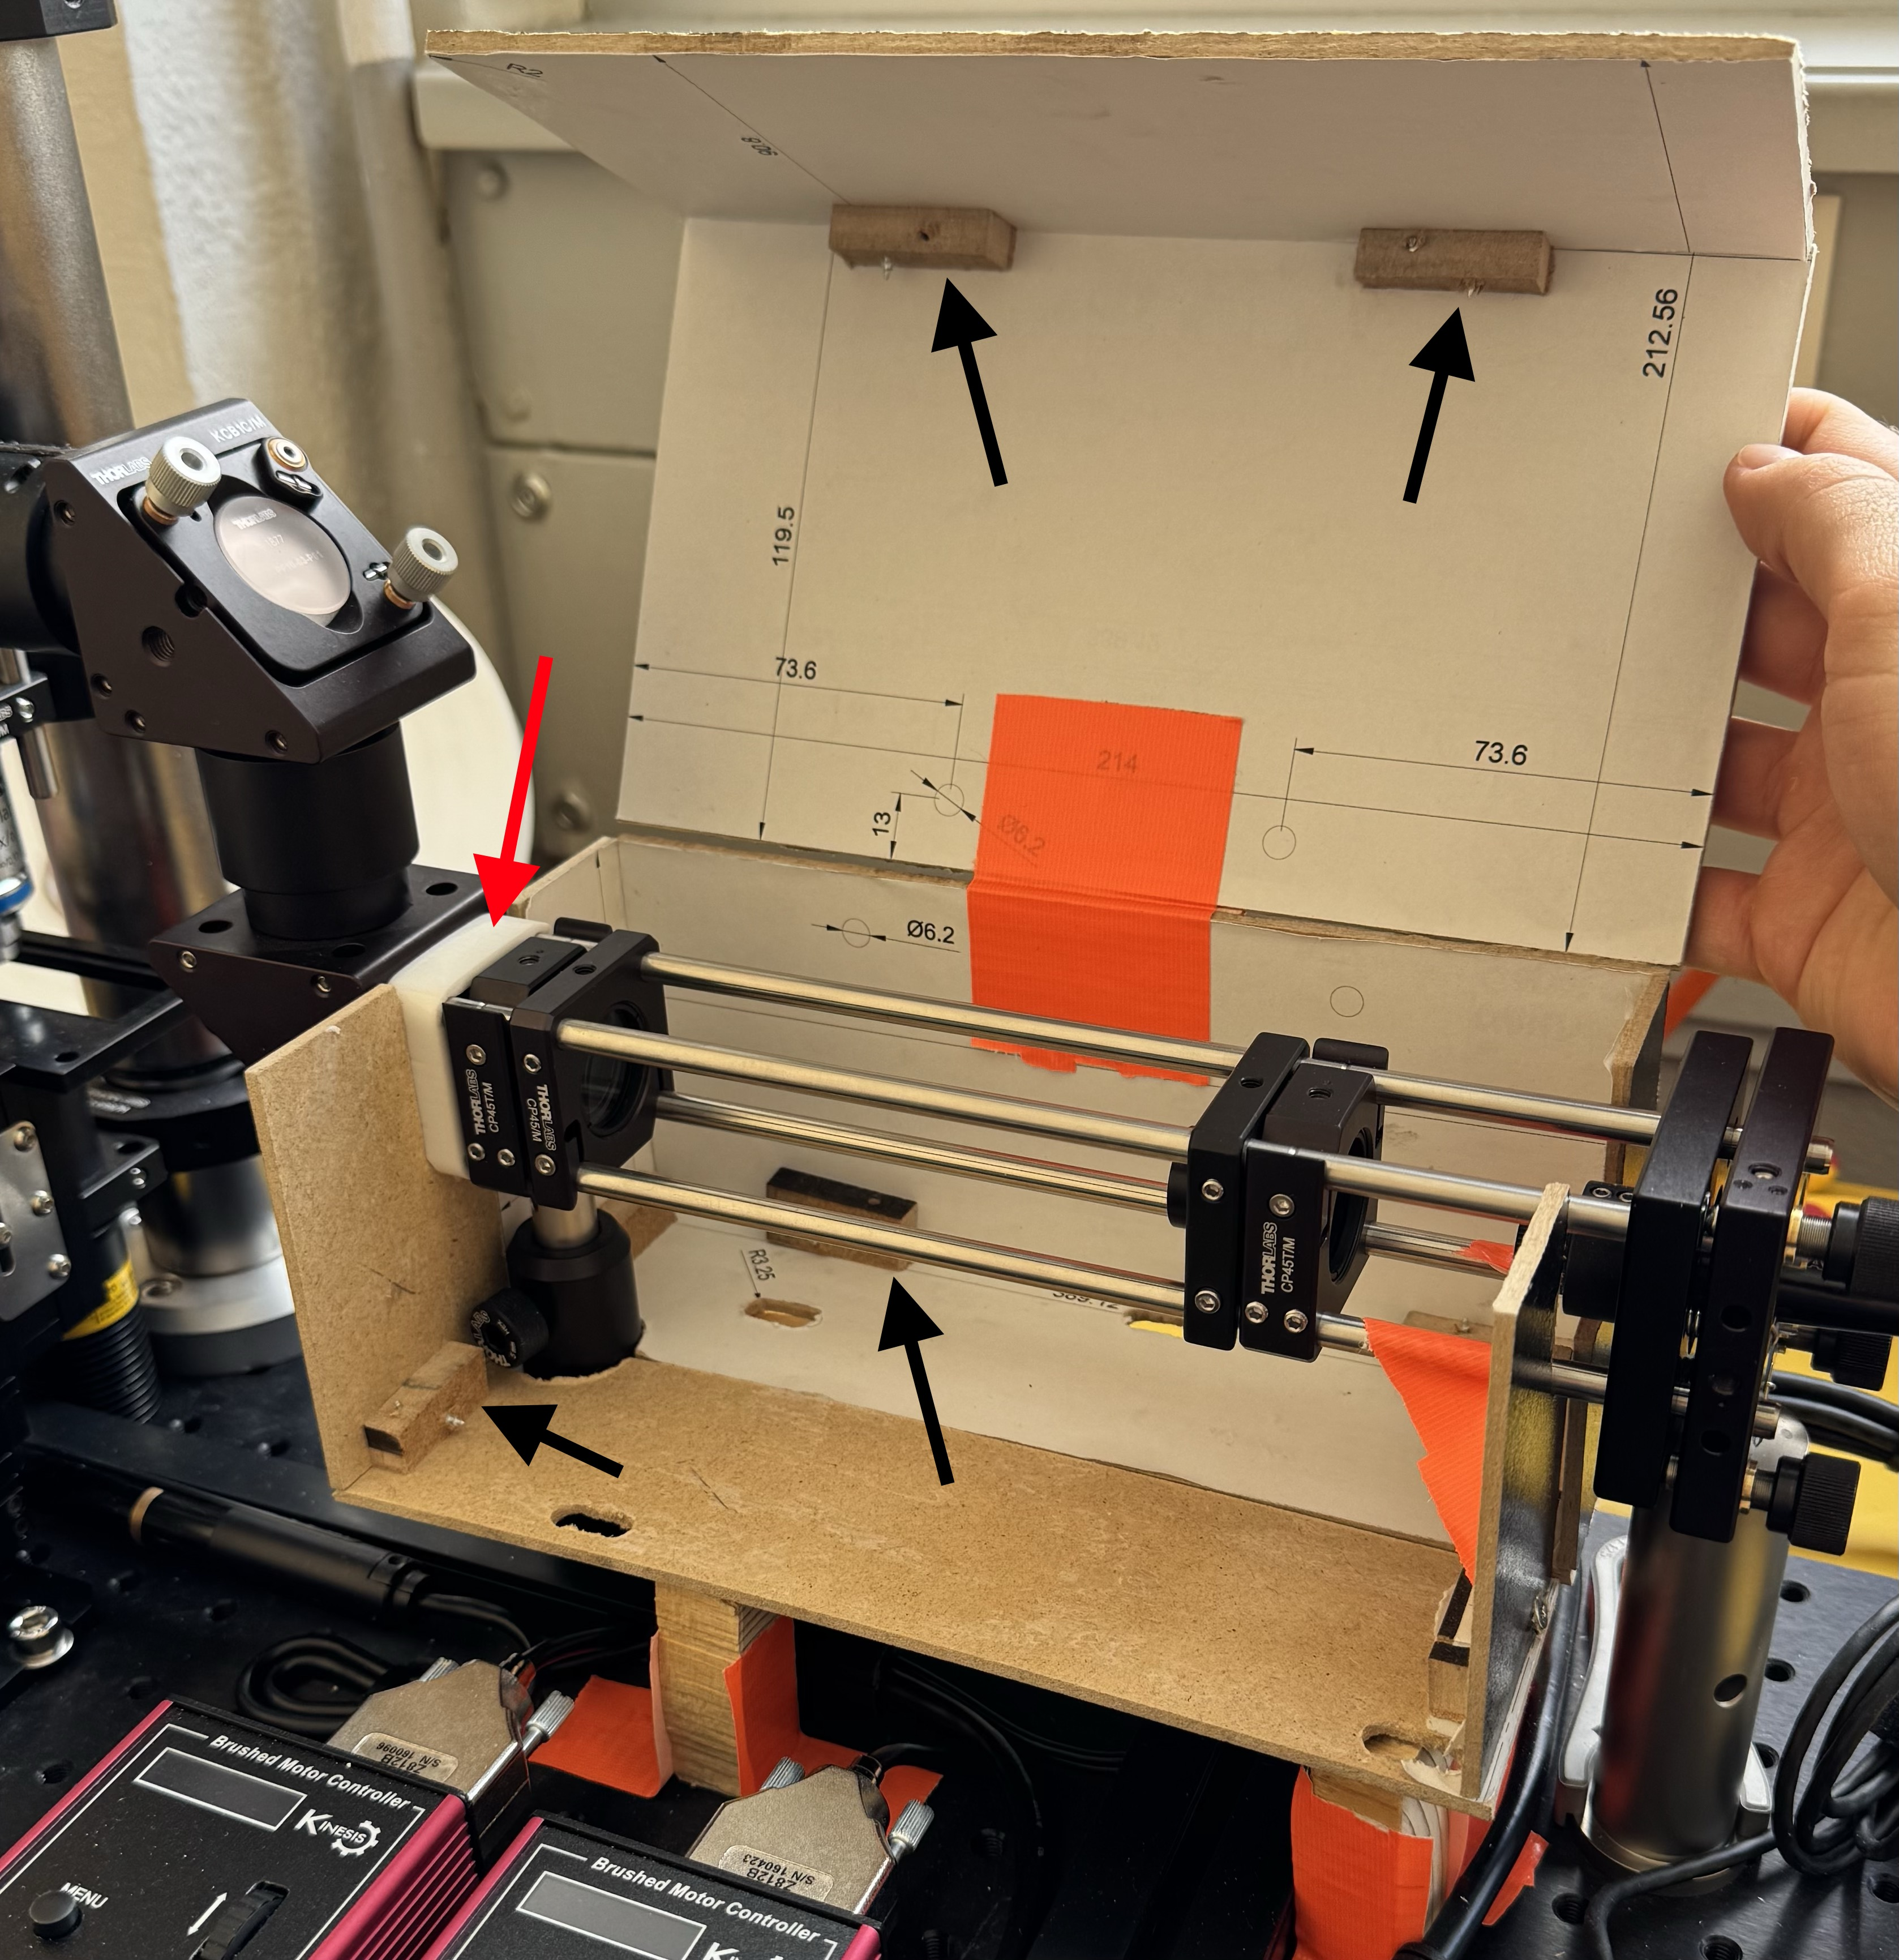
\includegraphics[width=0.6\textwidth]{assets/figures/Protections_laser/Securite_mecanique/Protection_entree_laser/montage_bois.jpeg}
    \end{center}
    \captionof{figure}{Montage de la protection à l'entrée du laser en bois MDF de 3~mm}
    \label{montage_bois}
\end{minipage}
\subsection{Fabrication des pièces en aluminium}
\begin{minipage}{\textwidth}

    \begin{minipage}[c]{0.6\textwidth}
        La Figure~\ref{capots_brutes} ci-contre, montre les trois pièces usinées par l'atelier mécanique, telles que reçues. Une peinture noire mat vient recouvrir les pièces pour absorber les rayons du laser.
    \end{minipage}\hfill
    \begin{minipage}[c]{0.35\textwidth}
        \begin{figure}[H]
            \centering
            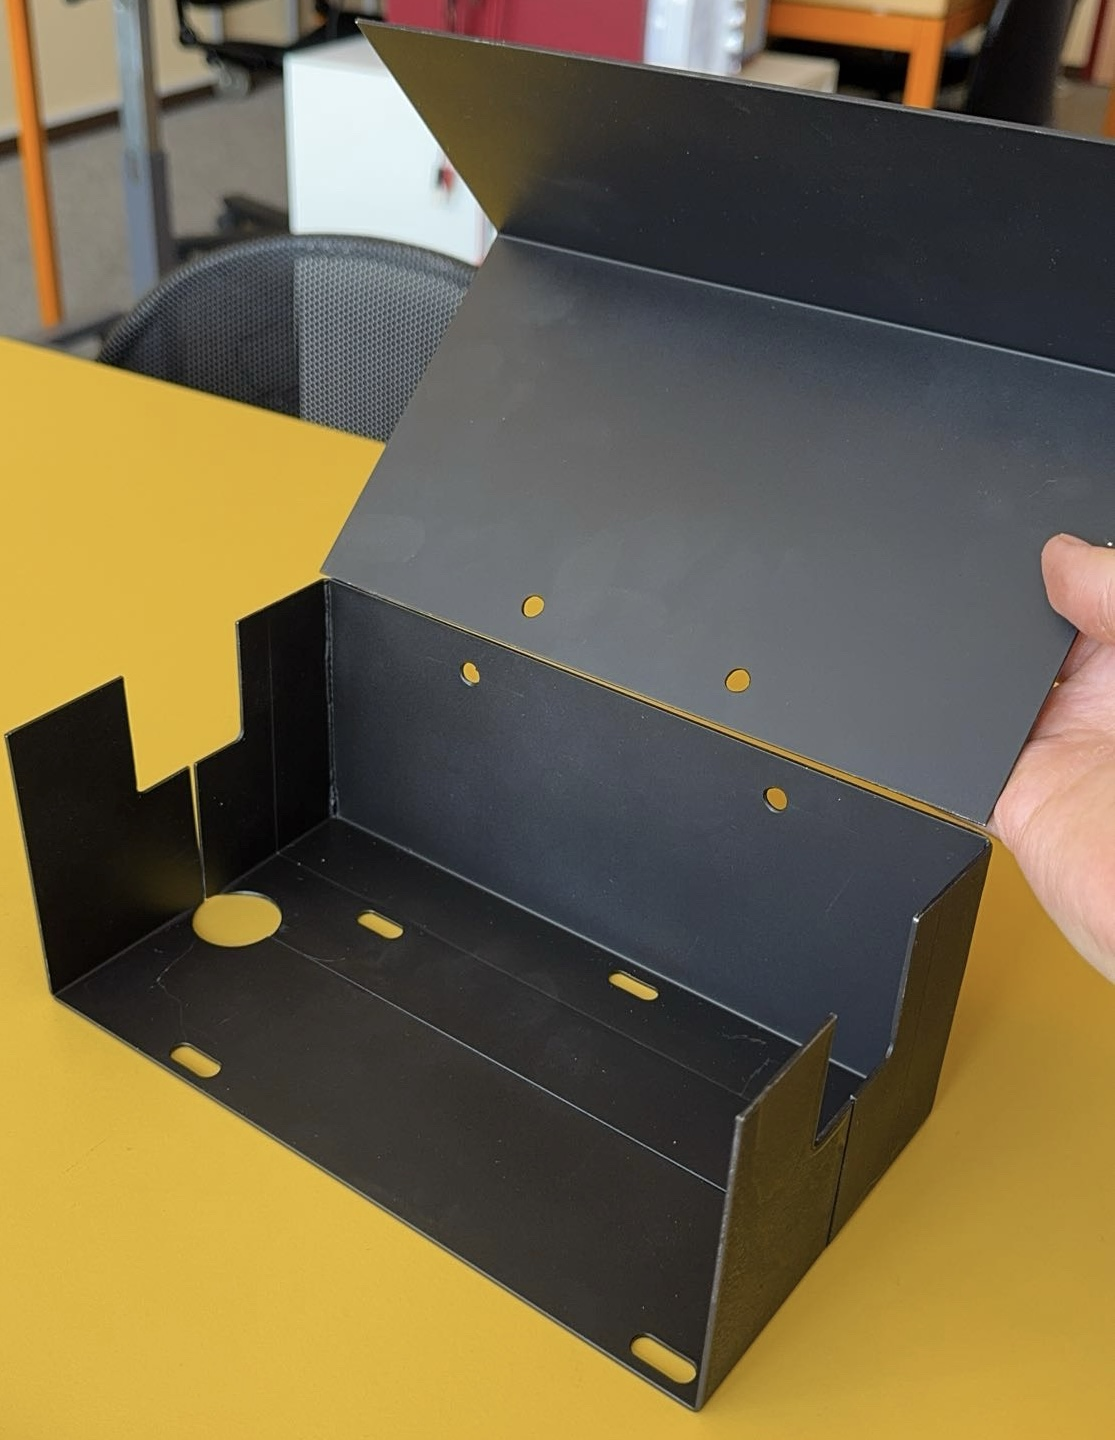
\includegraphics[width=\textwidth]{assets/figures/Protections_laser/Securite_mecanique/Protection_entree_laser/capots_brutes.jpg}
            \caption{Les trois protections fabriquées en aluminium 1.5~mm d'épaisseur}
            \label{capots_brutes}
        \end{figure}
    \end{minipage}
\end{minipage}


\begin{minipage}{\textwidth}
    \subsection{Montage final} \label{montage_final}
    Les figures~\ref{montage_alu_ouvert}~et~\ref{montage_alu_ferme} ci-dessous, représente le montage final des trois capots sur le kit.
    \vspace{1em}

    \begin{minipage}[c]{0.48\textwidth}
        \begin{figure}[H]
            \begin{center}
                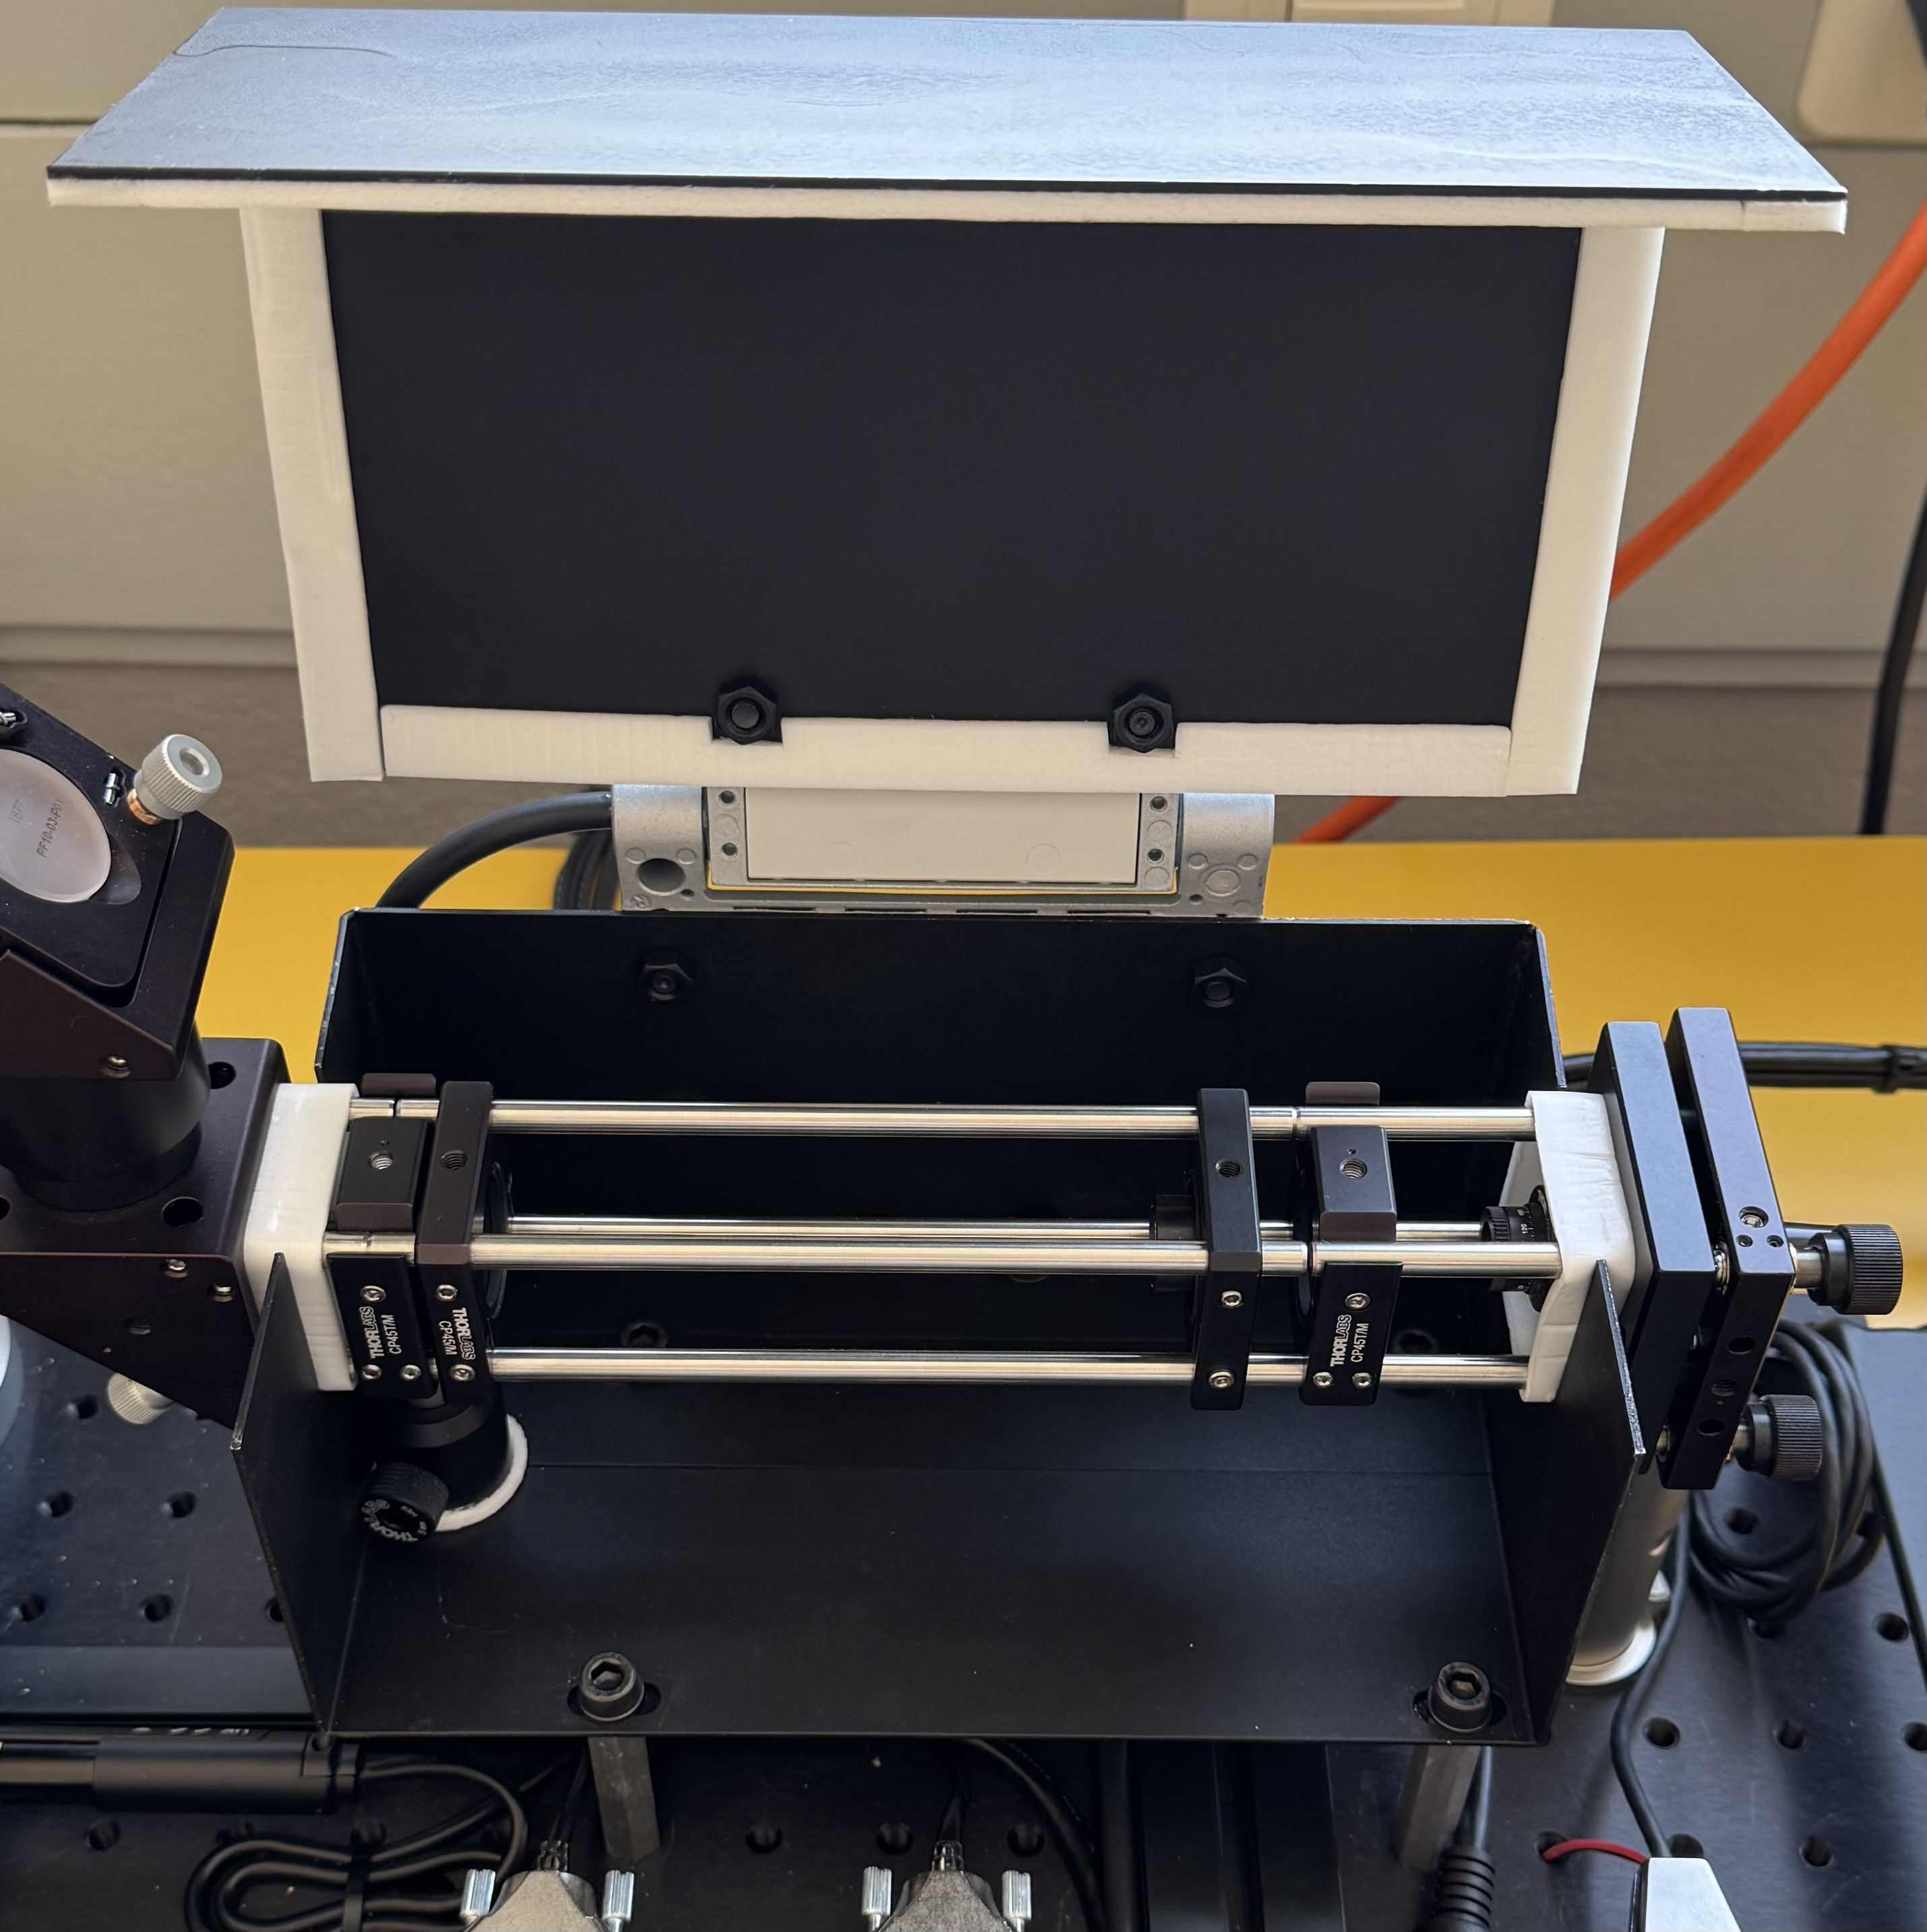
\includegraphics[height=6cm]{assets/figures/Protections_laser/Securite_mecanique/Protection_entree_laser/montage_alu_ouvert.jpeg}
            \end{center}
            \captionof{figure}{Montage de la protection \\ en aluminium: ouvert}
            \label{montage_alu_ouvert}
        \end{figure}
    \end{minipage}
    \begin{minipage}[r]{0.48\textwidth}
        \begin{figure}[H]
            \begin{center}
                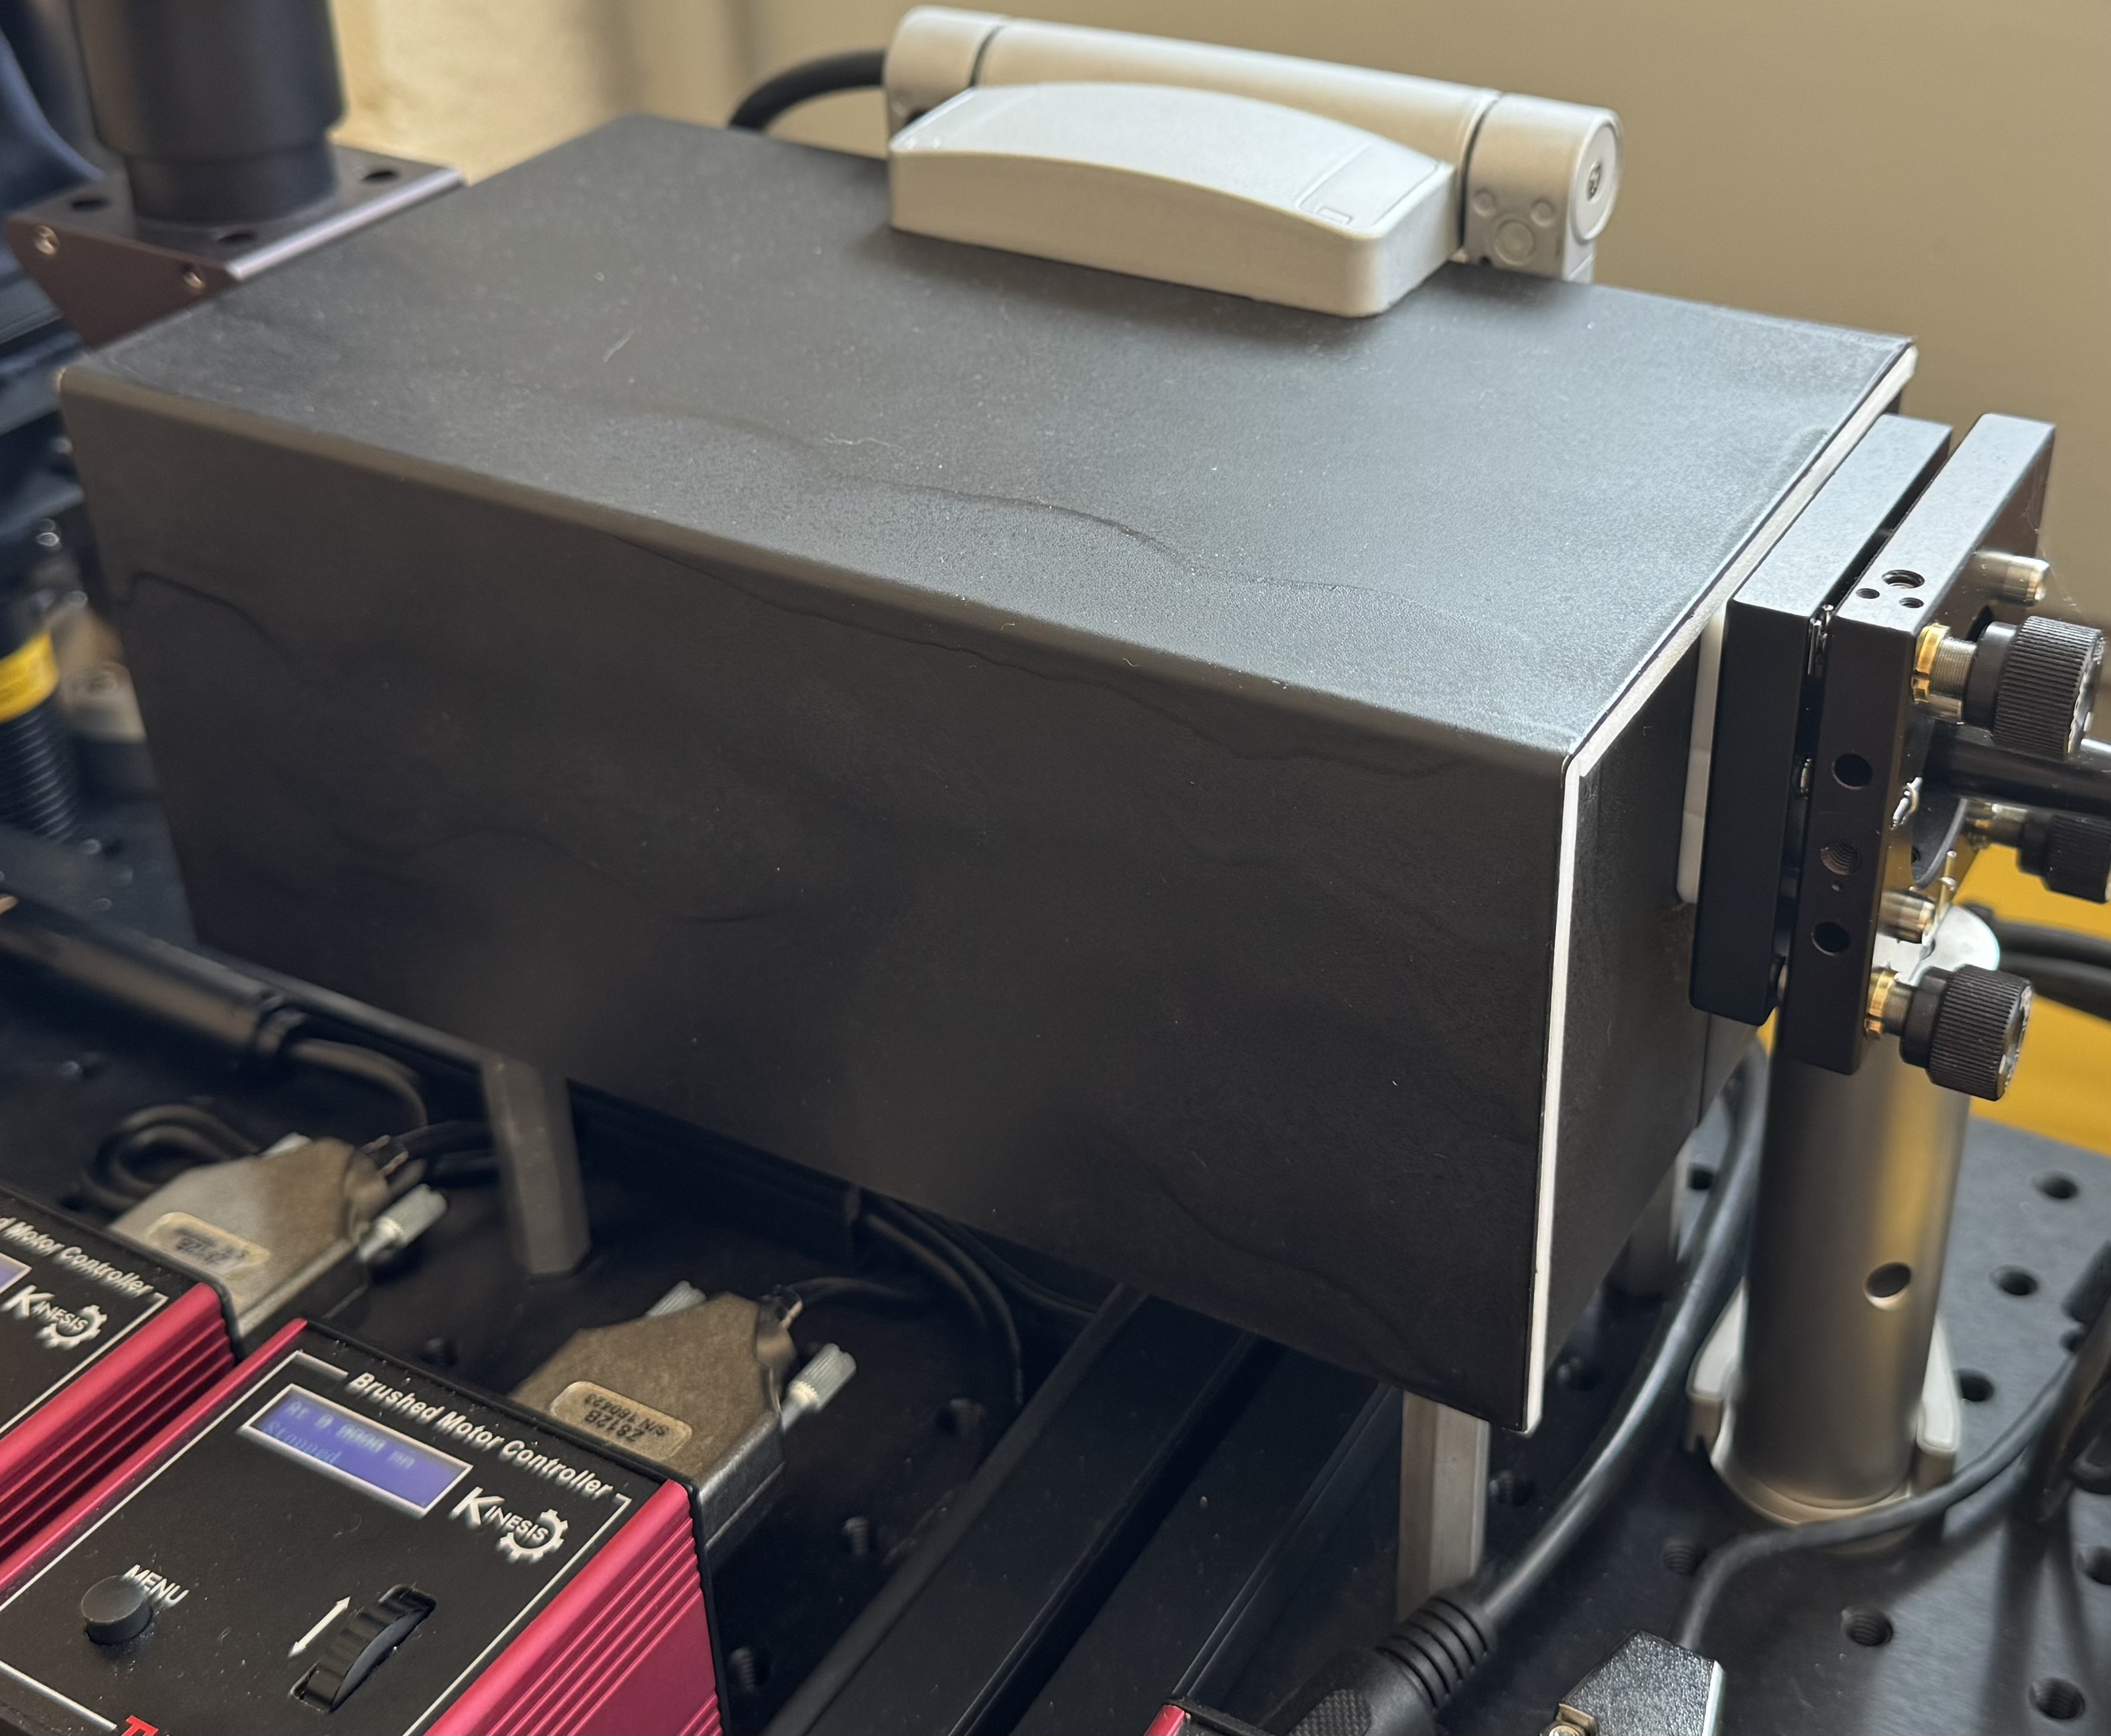
\includegraphics[height=6cm]{assets/figures/Protections_laser/Securite_mecanique/Protection_entree_laser/montage_alu_ferme.jpeg}
            \end{center}
            \captionof{figure}{Montage de la protection en aluminium: fermé}
            \label{montage_alu_ferme}
        \end{figure}
    \end{minipage}
\end{minipage}

\begin{minipage}{\textwidth}
    % La table ~\ref{tab:visserie_protection}, ci-dessous, liste l'ensemble de la visserie nécessaire pour le montage des protections sur le kit.

    % Prompt ChatGPT pour la création du tableau:
    % Fais moi un tableau récapitulatif de toute la visserie nécessaires:

    % - 5 vis imbus M6x20 pour fixer les entretoises à la platine.
    % - 5 vis imbus M6x8 pour fixer les tôles sur les entretoises.
    % - 5 rondelles M6.
    % - 4 vis imbus M6x16 pour fixer la charnière aux tôles.
    % - 4 écrous M6 pour la charnière

    \begin{table}[H]
        \centering
        \renewcommand{\arraystretch}{1.3}
        \begin{tabular}{|l|c|l|}
            \hline
            \textbf{Élément} & \textbf{Quantité} & \textbf{Utilisation}                                   \\
            \hline
            Vis imbus M6x20  & 5                 & Fixation des entretoises à la plaque de montage en alu \\
            Vis imbus M6x8   & 5                 & Fixation des tôles sur les entretoises                 \\
            Rondelles M6     & 5                 & Avec les vis M6x8                                      \\
            Vis imbus M6x16  & 4                 & Fixation de la charnière aux tôles                     \\
            Écrous M6        & 4                 & Pour les vis de la charnière                           \\
            \hline
        \end{tabular}
        \caption{Visserie nécessaire au montage de la protection. \cite{chatgptTableProtectionEntreeLaserVisserie}}
        \label{tab:visserie_protection}
    \end{table}
\end{minipage}
\subsection{Points d'améliorations}
\begin{enumerate}
    \item Les oblongs ne sont pas nécessaires. Au montage, je me suis rendu compte qu'en vissant les protections, la rondelle ne couvrait pas entièrement les oblongs. De ce fait, un jour subsistait. J'ai ajouté du scotch noir afin de combler ces espaces.
    \item La conception de la protection peut sûrement être améliorée. Par exemple, il serait éventuellement possible de réduire le nombre de fixations, afin de gagner en ergonomie.
\end{enumerate}
\clearpage
\section{Protection vers le microscope}
Cette section va expliquer les différentes étapes de la conception de la protection vers le microscope, la
modélisation de celle-ci, les prototypes qui ont été réalisés, la fabrication final ainsi
que le montage.
\subsection{Réflexion préliminaire}
Contrairement à la précédente protection, la table croisée bouge dans l'espace sur les trois axes X,Y et Z. Il faut, dans ce cas, trouvé un moyen de faire une protection qui puisse être mobile afin de supporter les efforts dans toutes les directions. La table peut se déplacer d'environ 12~mm en X et Y, et de 25~mm en Z.

La première approche s'est tournée vers de l'impression 3D de plastique souple, tel que du TPU. Ses propriétés élastiques permettent d'avoir une certaine liberté de mouvement.

Les Figures~\ref{zigzag_model}~et~\ref{zigzag_reel} ci-dessous, illustrent un modèle 3D de test avec une géométrie en \textit{zigzag}, afin de tester ses propriétés élastiques. Ce modèle n'a pas du tout été concluant, la structure est beaucoup trop rigide en élasticité et au contraire.

\begin{minipage}[c]{0.48\textwidth}
    \begin{center}
        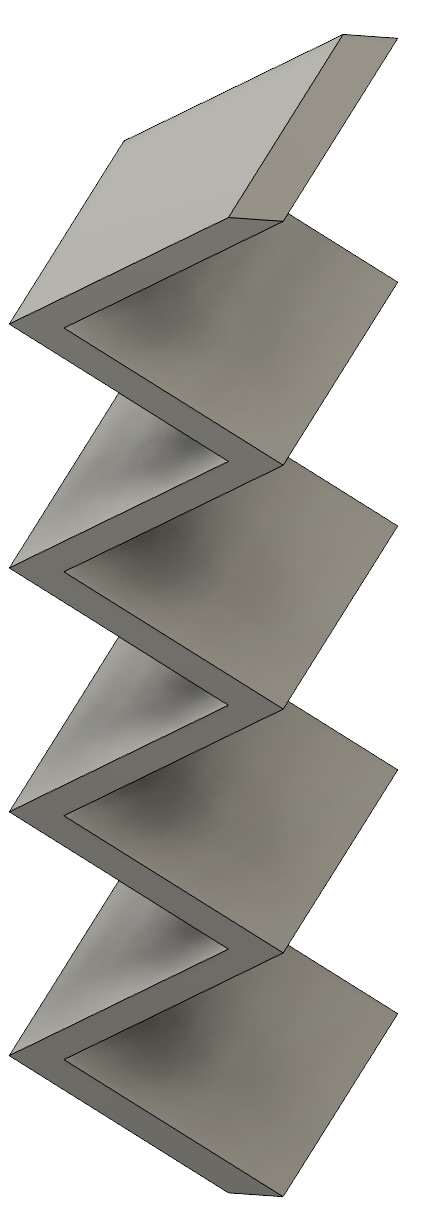
\includegraphics[width=0.2\textwidth]{assets/figures/Protections_laser/Securite_mecanique/Protection_vers_microscope/zigzag_model.jpeg}
    \end{center}
    \captionof{figure}{Modèle 3D avec géométrie en zigzag}
    \label{zigzag_model}
\end{minipage}\hfill
\begin{minipage}[c]{0.48\textwidth}
    \begin{center}
        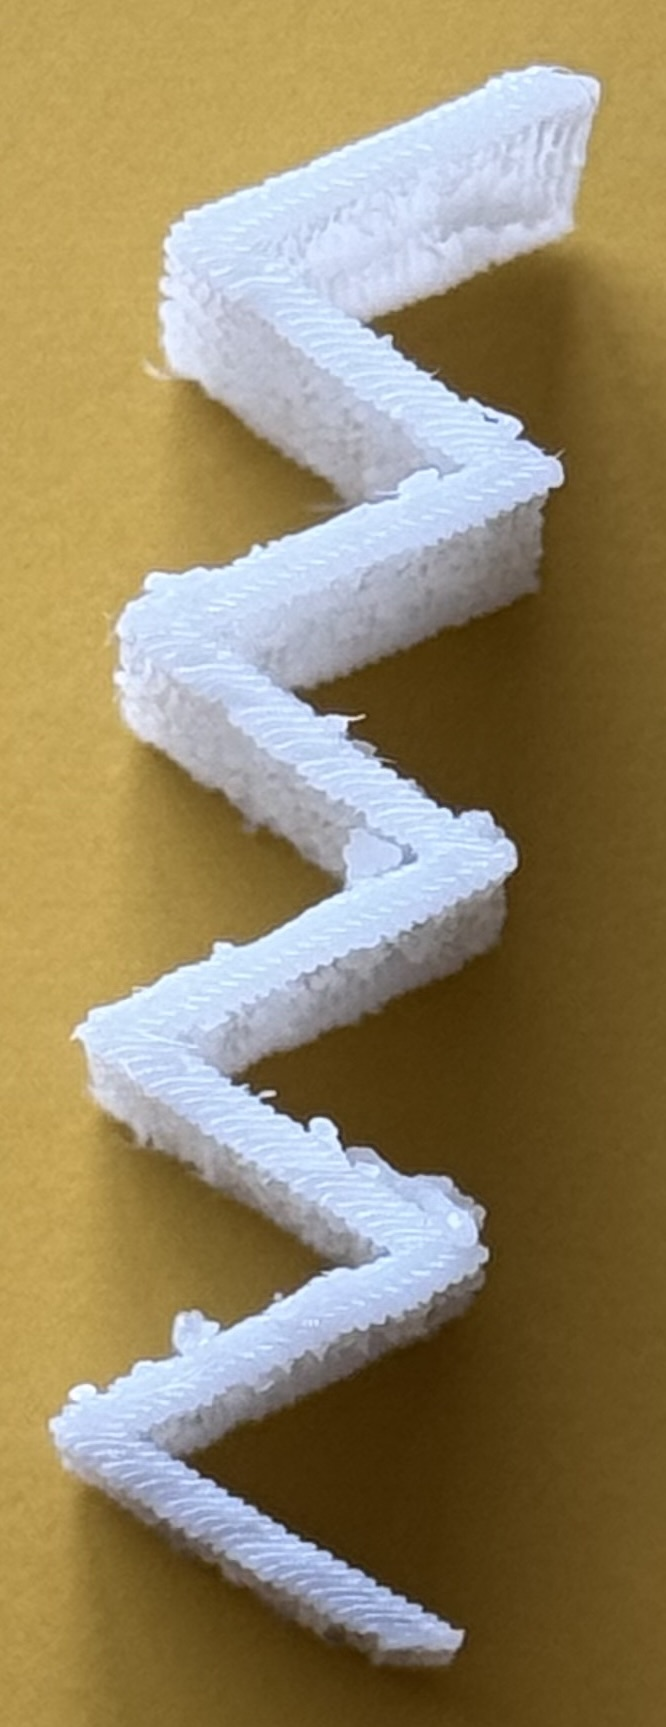
\includegraphics[width=0.2\textwidth]{assets/figures/Protections_laser/Securite_mecanique/Protection_vers_microscope/zigzag_reel.jpeg}
    \end{center}
    \captionof{figure}{Impression 3D en TPU du modèle avec géométrie en zigzag}
    \label{zigzag_reel}
\end{minipage}

La solution retenu pour avoir le moins de contraintes possible dans les mouvements a été de faire une conception de protection avec du tissu, associée à des impressions 3D en PLA.

\subsection{Modélisation de la protection}
\begin{minipage}[c]{0.38\textwidth}
    Pour pouvoir mieux comprendre les choix de conception et les étapes faites pour réaliser la protection, la Figure~\ref{model_3D_microscope}, ci-contre, représente la modélisation complète de la protection vers le microscope. Les modélisation crées pour cette protection sont en couleur sur la représentation 3D.
\end{minipage}\hfill
\begin{minipage}[c]{0.58\textwidth}
    \begin{center}
        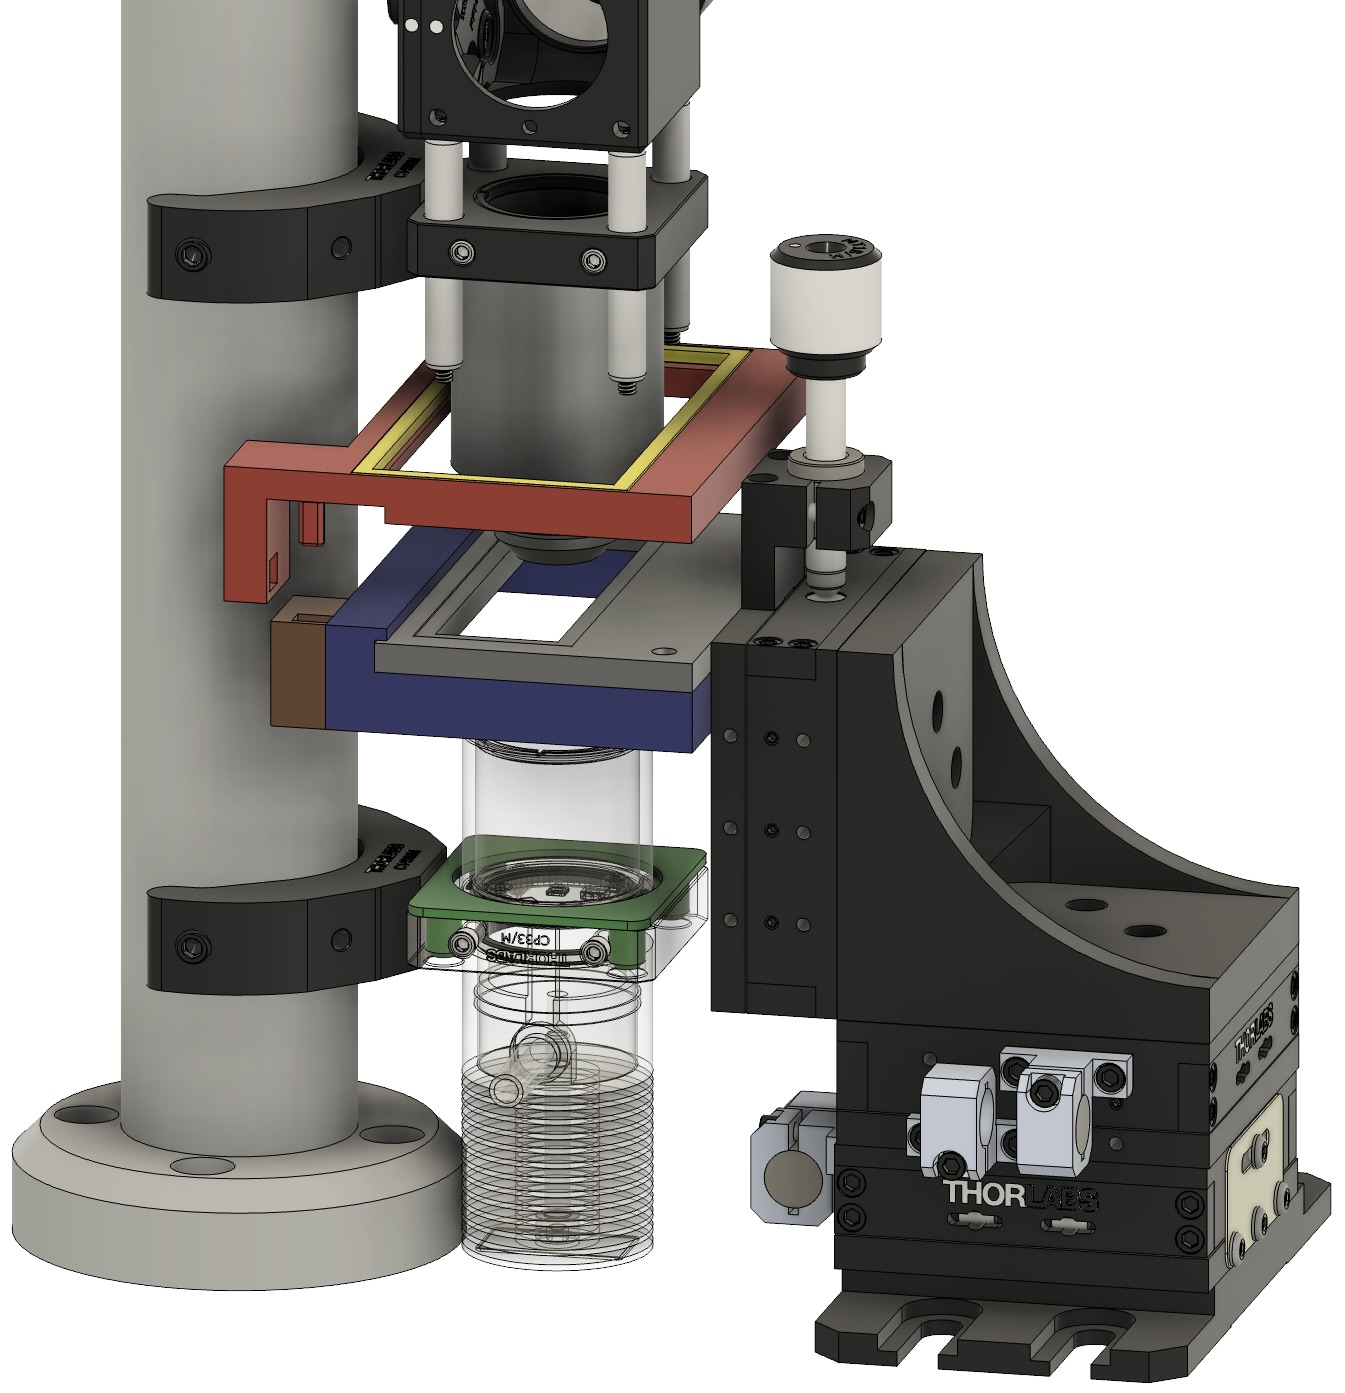
\includegraphics[width=\textwidth]{assets/figures/Protections_laser/Securite_mecanique/Protection_vers_microscope/model_3D.jpeg}
    \end{center}
    \captionof{figure}{Modèle 3D complet de la protection vers le microscope}
    \label{model_3D_microscope}
\end{minipage}

% Prompt ChatGPT pour la création du tableau:
% Fais moi un tableau avec les éléments ci-dessous:

% Partie inférieure:
% - En vert, support pour fixer le tissu inférieur à la LED
% - En bleu foncé, support pour fixer le tissu inférieur à la platine
% Partie supérieure:
% - En rouge, support qui vient se clipser sur la platine
% - En brun, boitier pour fixer le fin de course
% - En jaune, cadre pour fixer le tissu supérieur au support rouge

\begin{table}[H]
    \centering
    \begin{tabular}{|c|l|}
        \hline
        \textbf{Couleur}                         & \textbf{Nom de la pièce}                             \\
        \hline
        \multicolumn{2}{|c|}{\textbf{Partie inférieure}}                                                \\
        \hline
        \textcolor[RGB]{70, 170, 70}{Vert}       & Support pour fixer le tissu inférieur à la LED       \\
        \textcolor[RGB]{30, 50, 150}{Bleu foncé} & Support pour fixer le tissu inférieur à la platine   \\
        \hline
        \multicolumn{2}{|c|}{\textbf{Partie supérieure}}                                                \\
        \hline
        \textcolor[RGB]{170, 50, 50}{Rouge}      & Support clipsable sur la platine                     \\
        \textcolor[RGB]{120, 70, 30}{Brun}       & Boîtier pour fixer le fin de course                  \\
        \textcolor[RGB]{233, 173, 56}{Jaune}     & Cadre pour fixer le tissu supérieur au support rouge \\
        \hline
    \end{tabular}
    \caption{Nomenclature des pièces modélisées avec code couleur pour la protection vers le microscope. \cite{chatgptTableProtectionVersMicroscope}}
    \label{tab:nomenclature_pieces_microscope}
\end{table}

\subsubsection{Partie inférieure}
\begin{minipage}[c]{0.48\textwidth}
    Pour fixer le tissu à LED (pièce \textcolor[RGB]{70, 170, 70}{verte} de la Figure~\ref{model_3D_microscope}), le support montré sur la Figure~\ref{support_inf_tissu_LED}, ci-contre, a été pensé. La plaque, désigné par la flèche \textcolor{red}{rouge}, est une plaque de cage.
    \vspace{1em}
    Ses quatres trous ont été utilisés pour pouvoir fixer le support. les quatres petites vis (flèches \textcolor[RGB]{115, 210, 210}{bleues}), sont des vis sans têtes pour serrer le support en place. Le tissu est pincé entre la plaque et le support imprimé.
\end{minipage}\hfill
\begin{minipage}[c]{0.48\textwidth}
    \begin{center}
        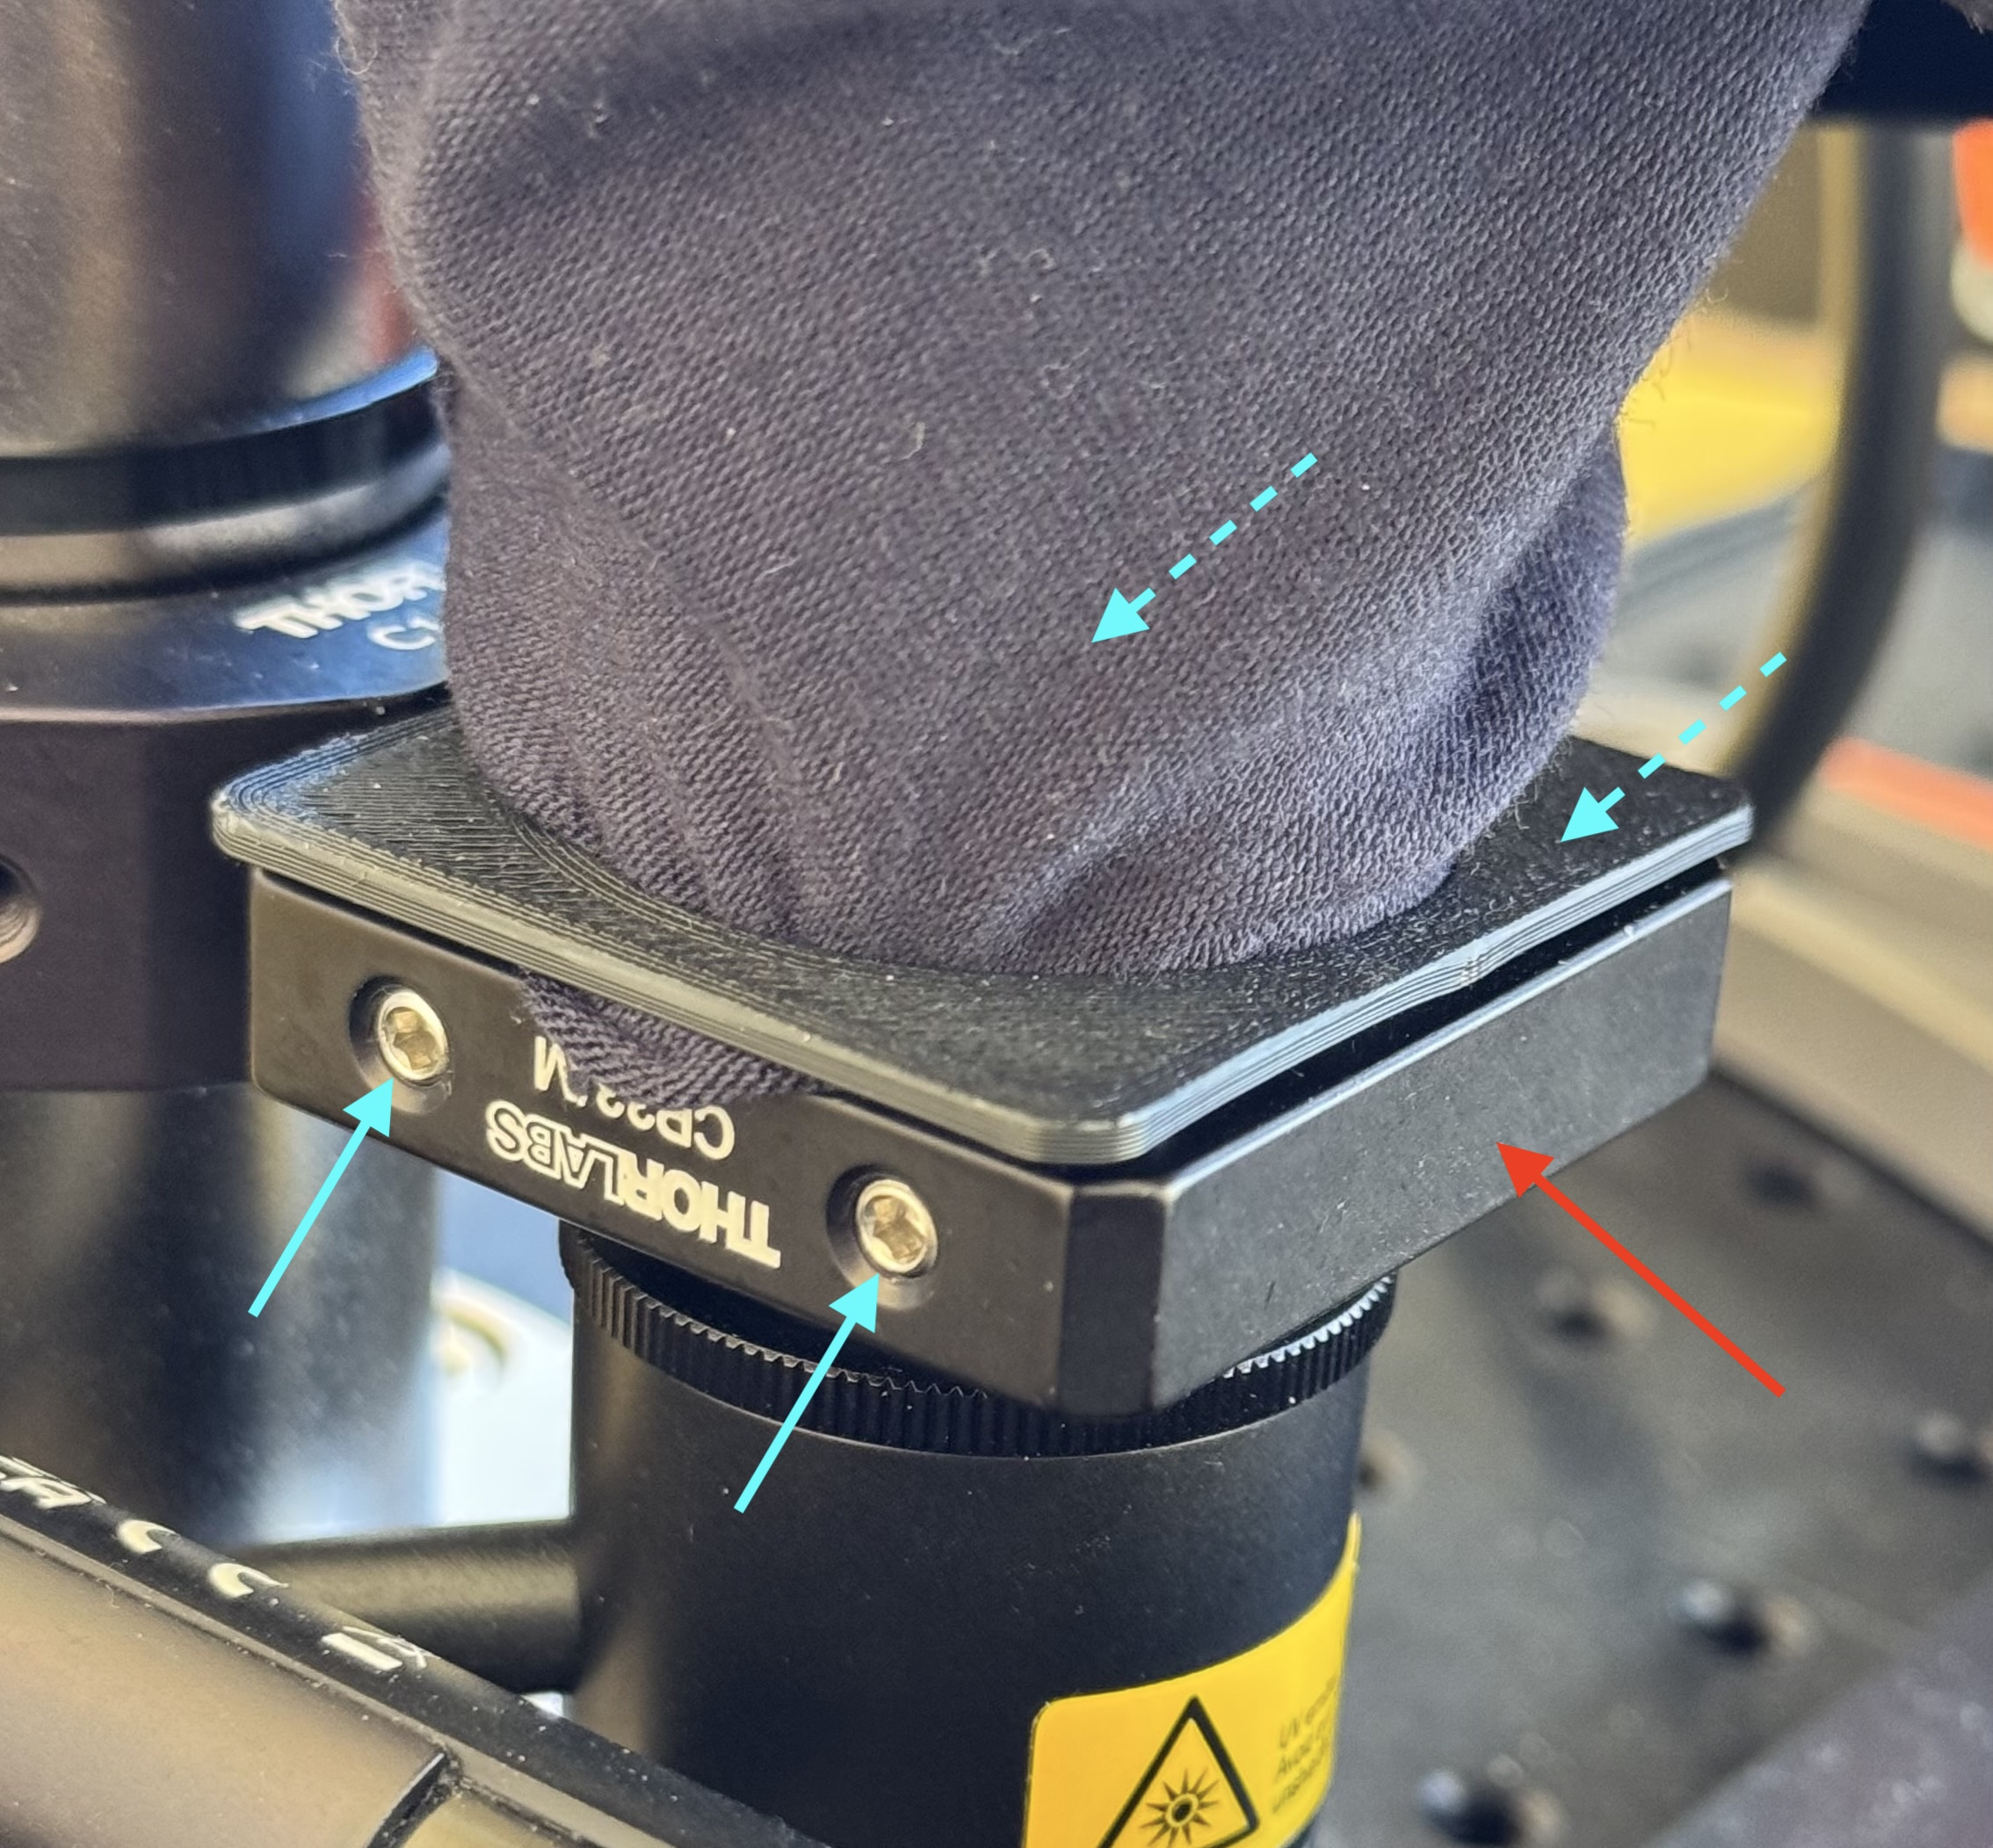
\includegraphics[width=0.9\textwidth]{assets/figures/Protections_laser/Securite_mecanique/Protection_vers_microscope/support_inf_tissu_LED.jpeg}
    \end{center}
    \captionof{figure}{Support pour fixer le tissu inférieur à la lED}
    \label{support_inf_tissu_LED}
\end{minipage}

\begin{minipage}[c]{0.48\textwidth}
    Pour fixer le tissu à la platine (pièce \textcolor[RGB]{30, 50, 150}{bleu foncé} de la Figure~\ref{model_3D_microscope}), le support montré sur la Figure~\ref{support_inf_tissu_platine} (flèche \textcolor{red}{rouge}), ci-contre, a été élaboré.

    \vspace{1em}
    Pour le fixer, les vis montrées par les flèches \textcolor[RGB]{115, 210, 210}{bleues} ont été utilisées. Comme pour la fixation à la LED, ici, le tissu est également coincé entre la platine et le support.
\end{minipage}\hfill
\begin{minipage}[c]{0.48\textwidth}
    \begin{center}
        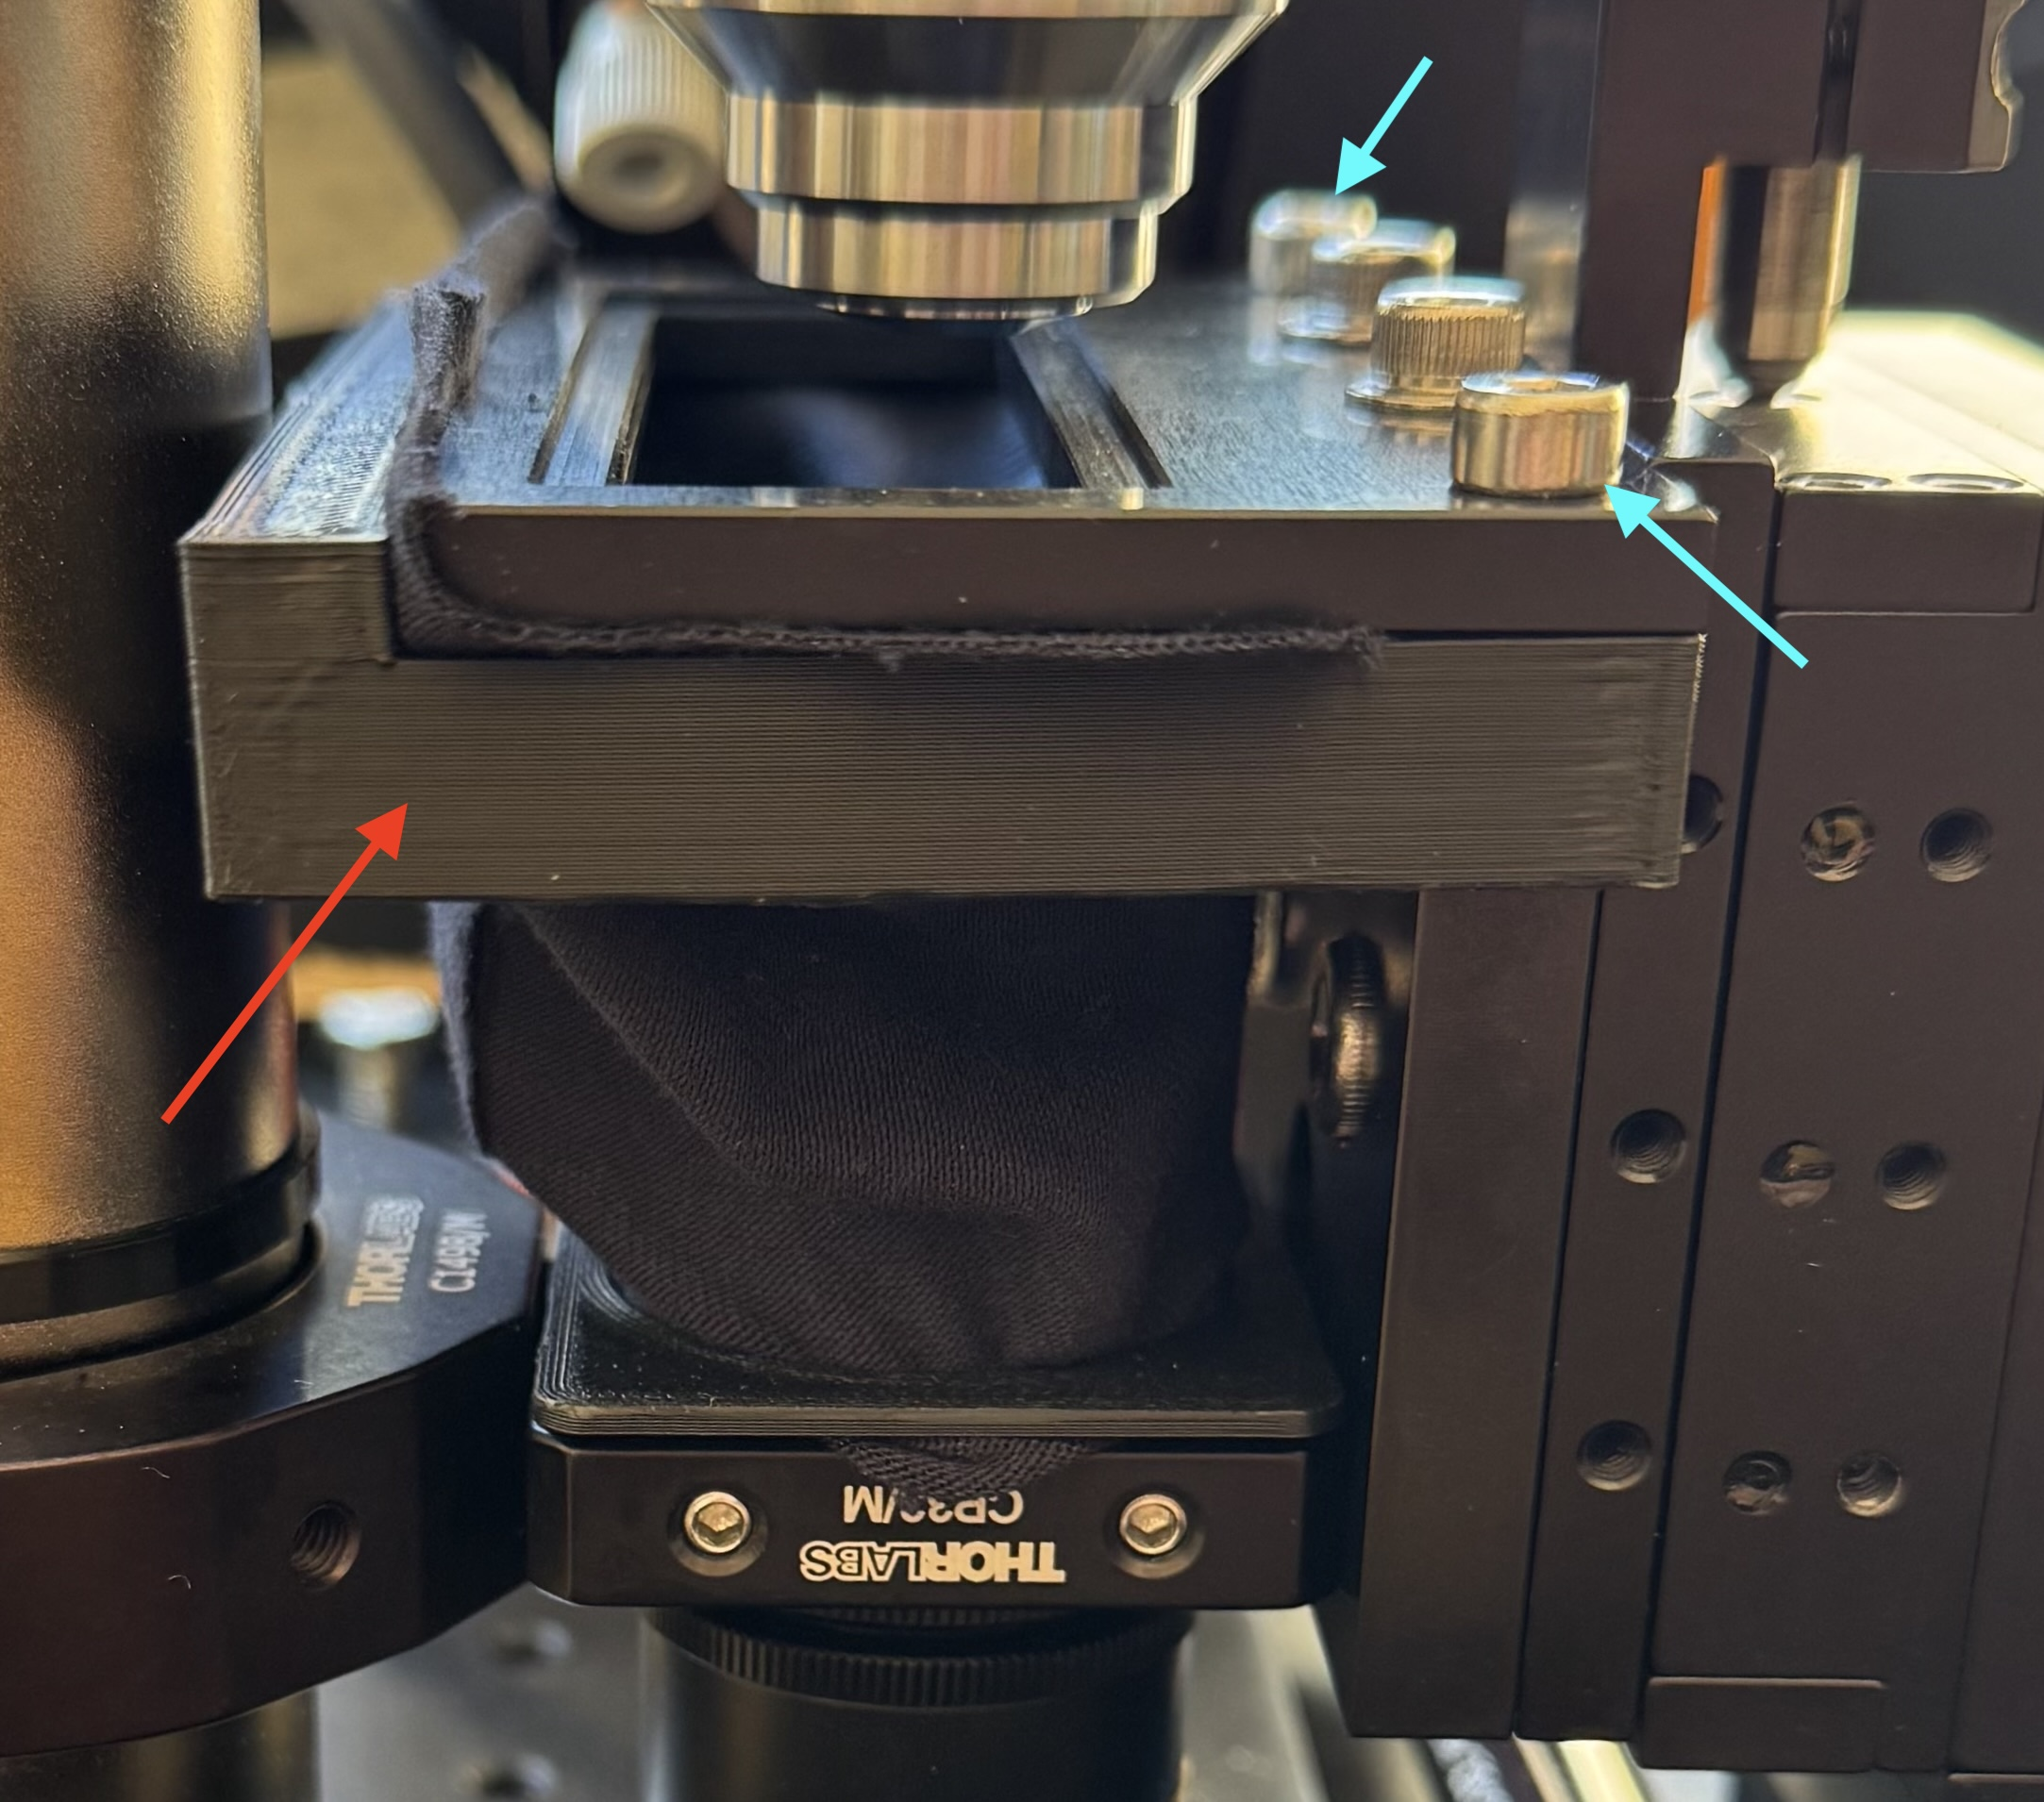
\includegraphics[width=0.9\textwidth]{assets/figures/Protections_laser/Securite_mecanique/Protection_vers_microscope/support_inf_tissu_platine.jpeg}
    \end{center}
    \captionof{figure}{Support pour fixer le tissu inférieur à la platine}
    \label{support_inf_tissu_platine}
\end{minipage}

\subsubsection{Partie supérieure}

\begin{minipage}[c]{0.48\textwidth}
    Pour la partie supérieure, la fixation du tissu est assuré avec le cadre \textcolor[RGB]{233, 173, 56}{jaune} et le support \textcolor[RGB]{170, 50, 50}{rouge} illustré sur la Figure~\ref{model_3D_microscope}. Ce support imprimé est montré par la flèche \textcolor{red}{rouge} sur cette Figure~\ref{support_sup_tissu_microscope} ci-contre.

    \vspace{1em}
    Pour fixer le tissu à la structure au-dessus du microscope, une simple attache rapide (flèche \textcolor[RGB]{115, 210, 210}{bleue}) a été utilisé pour le maintenir en place.

\end{minipage}\hfill
\begin{minipage}[c]{0.48\textwidth}
    \begin{center}
        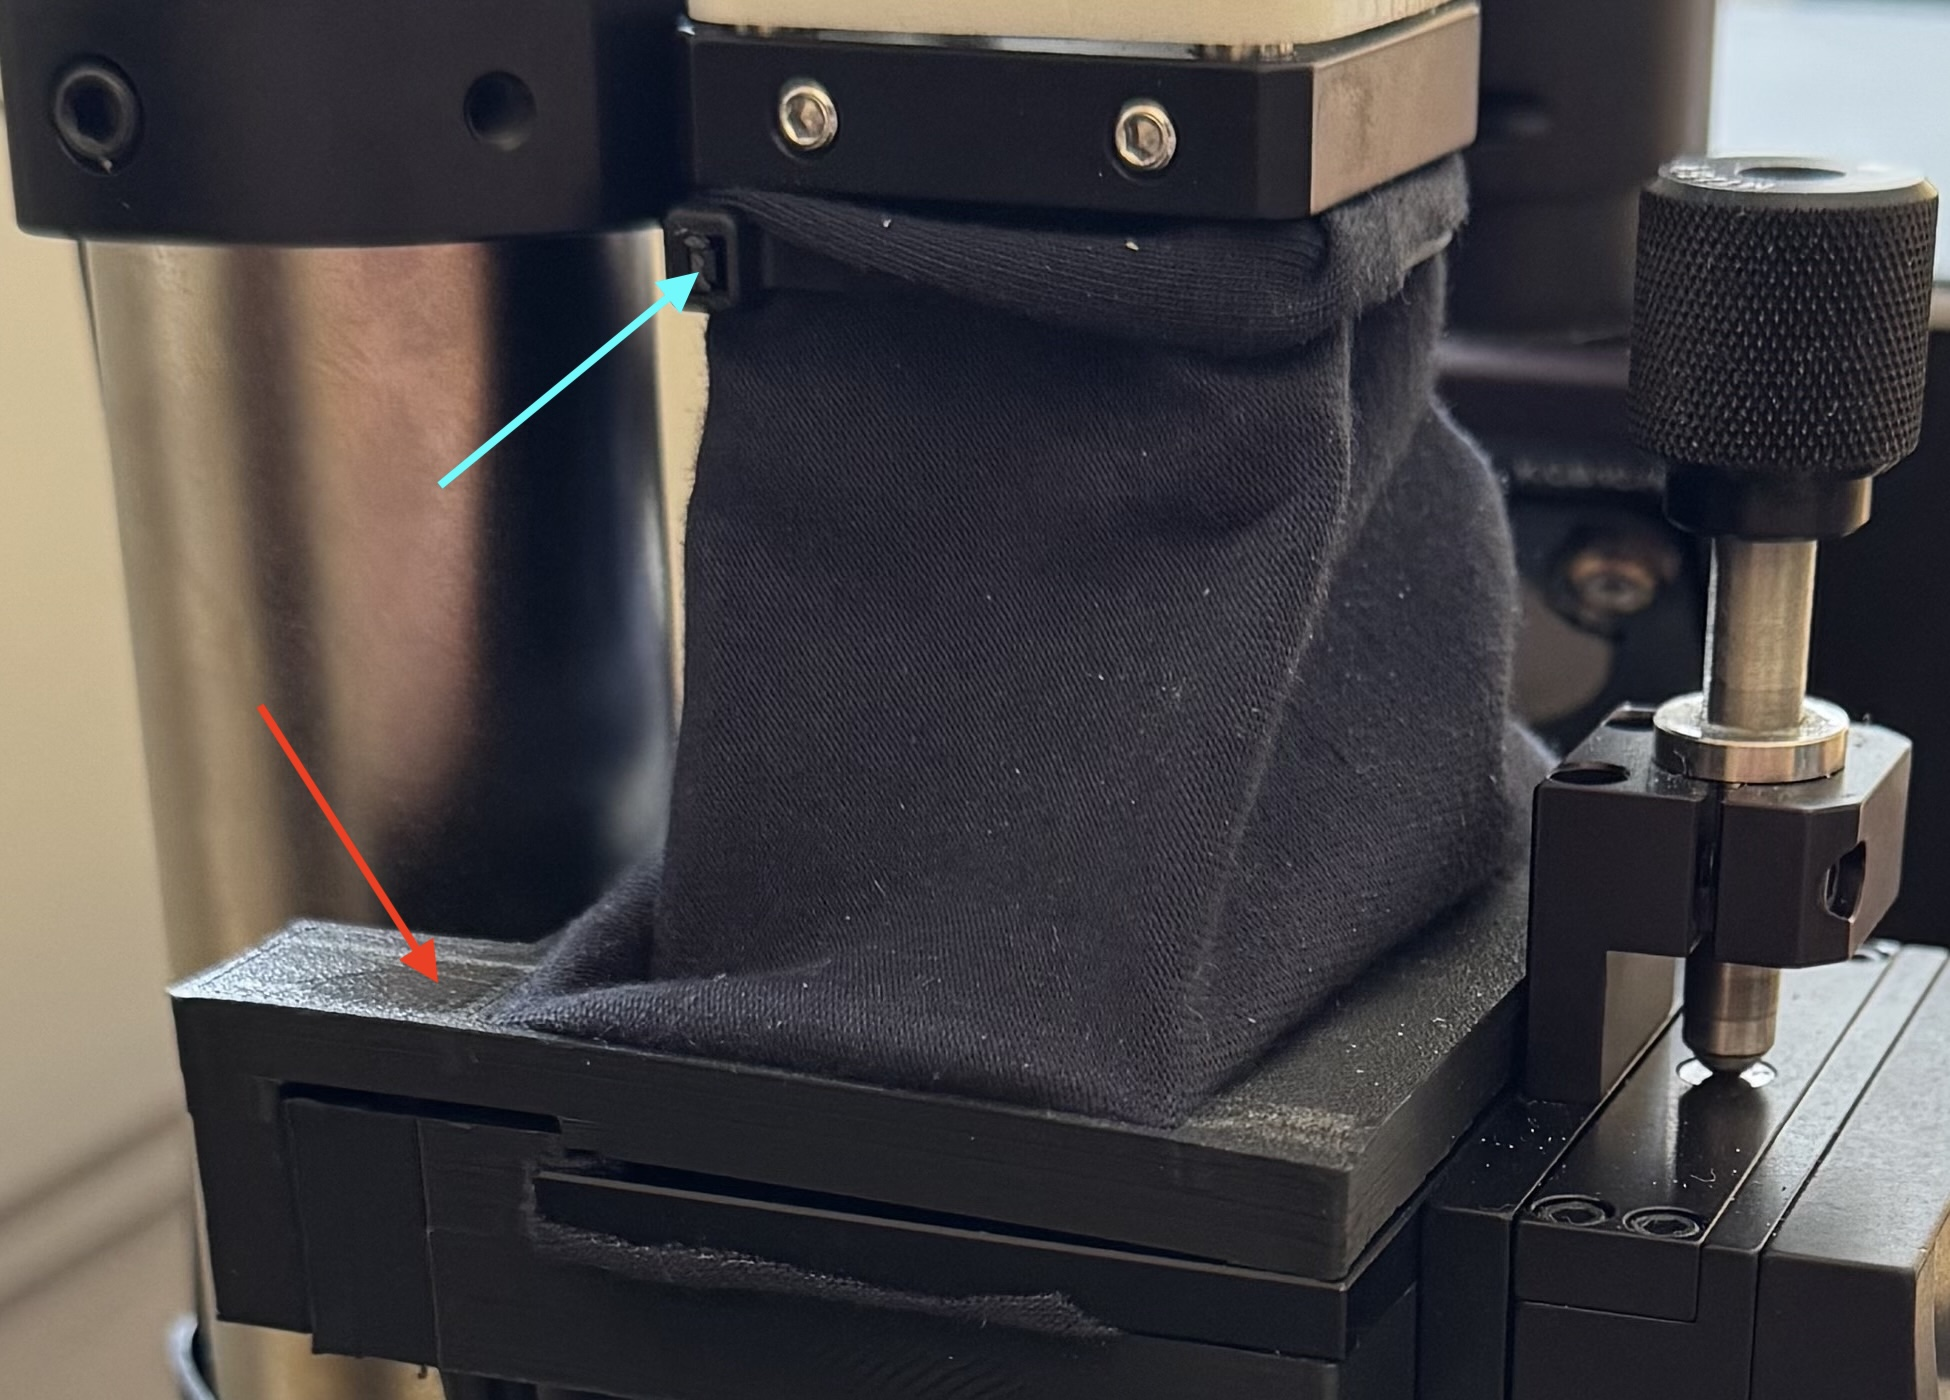
\includegraphics[width=0.9\textwidth]{assets/figures/Protections_laser/Securite_mecanique/Protection_vers_microscope/support_sup_tissu_microscope.jpeg}
    \end{center}
    \captionof{figure}{Support pour fixer le tissu inférieur à la platine}
    \label{support_sup_tissu_microscope}
\end{minipage}

\subsubsection{Fin de course}
\begin{minipage}[c]{0.48\textwidth}
    Afin d'assurer le bon fonctionnement du fin de course, le boîtier modélisé en \textcolor[RGB]{120, 70, 30}{brun} sur la Figure~\ref{model_3D_microscope}, a été créé. Son modèle imprimé est représenté par la flèche \textcolor[RGB]{115, 210, 210}{bleue} sur la Figure~\ref{boitier_fin_de_course}.

    \vspace{1em}
    L'axe, encadré en \textcolor[RGB]{233, 173, 56}{jaune}, assure l'actionnement du fin de course.

\end{minipage}\hfill
\begin{minipage}[c]{0.48\textwidth}
    \begin{center}
        \includegraphics[width=0.9\textwidth]{assets/figures/Protections_laser/Securite_mecanique/Protection_vers_microscope/boitier_fin_de_course.png}
    \end{center}
    \captionof{figure}{Boîtier pour le fin de course}
    \label{boitier_fin_de_course}
\end{minipage}

\subsection{Points d'améliorations}